\section{Electroweak Corrections in the Standard Model}
\label{sec:ew-sm}

After the inclusion of the higher-order QCD corrections and top quark mass effects discussed above, electroweak effects become a relevant ingredient of a precision prediction for Higgs boson pair production. They probe parts of the Standard Model dynamics that are complementary to QCD, including the top Yukawa interaction, weak gauge-boson contributions, and light-quark initiated channels. In this section we summarize the recent computation of the complete NLO electroweak corrections to the gluon-fusion process, compare it with separately studied subsets of the two-loop contributions, and discuss the small but shape-dependent quark-antiquark channel in the LHC setup relevant for this report.

%%\subsection{General features}

%\label{EW:common}

%From Huan-Yu Bi, Li-Hong Huang, Rui-Jun Huang, Yan-Qing Ma, Huai-Min Yu

The structure of the virtual NLO electroweak (EW) amplitude for double Higgs boson production from gluon fusion can be decomposed as~\cite{Bi:2023bnq}
\begin{align}
{\cal M}^{\mu\nu}=F_1T_1 ^{\mu\nu}+F_2T_2 ^{\mu\nu}+\Delta_0^{\mu\nu}+\Delta_5^{\mu\nu}
\,,
\label{eqref:decamplitudeEW}
\end{align}
assuming $p_{1,\mu}{\cal M}^{\mu\nu}=p_{2,\nu}{\cal M}^{\mu\nu}=0$. $\Delta_5^{\mu\nu}$ contains a single Levi-Civita tensor and appears from two loops onward, and $\Delta_0^{\mu\nu}$ depends on either $p_1^{\mu}$ or $p_2^{\nu}$. These two tensors will vanish when contracting the virtual NLO EW amplitude together with the LO amplitude. The physical tensors $T_1$ and $T_2$ are defined as in Section~\ref{intro_ampli}.

No real radiation is produced at NLO from EW corrections, thanks to Furry's theorem.



\subsection{Full SM electroweak corrections}

\label{EW:full}

\textbf{Huan-Yu Bi, Li-Hong Huang, Rui-Jun Huang, Yan-Qing Ma, Huai-Min Yu~\cite{Bi:2023bnq}.}

\noindent Ref.~\cite{Bi:2023bnq} identifies 116 integral families for the complete NLO EW corrections. The loop integrals in each family are reduced to master integrals using the {\tt Blade} package \cite{Blade}, employing {\tt FiniteFlow} \cite{Peraro:2019svx} to solve integration-by-parts (IBP) relations \cite{Chetyrkin:1981qh}, and incorporating a block-triangular form \cite{Liu:2018dmc,Guan:2019bcx} to enhance computational efficiency. Dimensional regularization is realized by choosing $\epsilon=\pm1/1000$, where $D=4-2\epsilon$. This eliminates the need for Laurent expansions in $\epsilon$ for computing the cross sections and thus reduces resource demands \cite{Liu:2022chg,Liu:2022mfb}. Master integrals are evaluated by numerically solving systems of differential equations \cite{Kotikov:1990kg,Remiddi:1997ny,Caffo:2008aw,Czakon:2008zk,Lee:2014ioa,Moriello:2019yhu,Hidding:2020ytt,Armadillo:2022ugh} in $\hat{s}$ and $\hat{t}$,  with boundary conditions computed using the {\tt AMFlow} package \cite{Liu:2022chg} implementing the auxiliary mass flow method \cite{Liu:2022mfb,Liu:2021wks,Liu:2017jxz}. The analytic continuation is performed by introducing an infinitesimal positive imaginary part to $\hat{s}$ to cross physical singularities arising in the master integrals, located at $\sqrt{\hat{s}}=2m_h$, $m_W+m_t$, $2m_t$, $2m_t+m_Z$, and $2m_t+m_h$, corresponding to intermediate particles going on-shell. The on-shell scheme for masses and fields is employed for the renormalization of the bare amplitudes, while the electromagnetic coupling $\alpha$ is renormalized in the $G_{\mu}$ scheme \cite{Denner:2019vbn}.

The cross section is obtained by integrating over the phase space,
\begin{align}\label{eq:Xsection}
\sigma^{\rm LO(NLO)} &= \frac{1}{512\pi}\int_0^1 \mathrm{d}x_{1}\int_0^1 \mathrm{d}x_{2} \int^{\hat{t}_{+}}_{\hat{t}_{-}}\mathrm{d}\hat{t} \,\times \nonumber \\
& \times \frac{1}{\hat{s}^{2}}f_{g/p}(x_{1},\mu)f_{g/p}(x_{2},\mu) M^{\rm LO(NLO)},
\end{align}
where $f_{g/p}(x,\mu)$ denotes the gluon distribution function of the proton, $\mu$ represents the factorization scale, $\hat{t}^{\pm}=m^{2}_{H}-\frac{\hat{s}}{2}(1\mp\sqrt{1-{4m^{2}_{H}}/{\hat{s}}})$, and $M^{\rm LO(NLO)}$ are given by
\begin{align}
M^{\rm LO}&=|F_{1}^{(0)}|^2+|F_{2}^{(0)}|^2 \;,\\
M^{\rm NLO}&=|F_{1}^{(0)}+F_{1}^{(1)}|^2-|F_{1}^{(1)}|^2\nonumber\\
&+|F_{2}^{(0)}+F_{2}^{(1)}|^2  -|F_{2}^{(1)}|^2,
\end{align}
where $F_i^{(0)}$ and $F_i^{(1)}$ correspond to the lowest order and the next-order terms in the $\alpha$ expansion of the form factors. The phase-space integration is carried out by optimized sampling techniques implemented through the {\tt Parni} package \cite{vanHameren:2007pt}.

The masses of the particles are set to
\begin{eqnarray}
\frac{m_h^2}{m_t^2}=\frac{12}{23}
\,,\qquad
\frac{m_Z^2}{m_t^2}=\frac{23}{83}
\,\qquad
\frac{m_W^2}{m_t^2}=\frac{14}{65}
\,,
\end{eqnarray}
with $m_t=172.69\,\textup{GeV}$ \cite{ParticleDataGroup:2022pth}. The electromagnetic coupling $\alpha=1/133.12=7.512\times 10^{-3}$ is derived from the Fermi constant $G_F=1.166378\times 10^{-5}\,\textup{GeV}^{-2}$ via
\begin{eqnarray}
\alpha=\frac{\sqrt{2}}{\pi}G_F m_W^2 \left(1-\frac{m_W^2}{m_Z^2}\right)
.
 \end{eqnarray}
The Cabibbo--Kobayashi--Maskawa (CKM) mixing matrix is set to be the unit matrix. The default PDF set for both LO and NLO calculations is NNPDF3.1 \cite{NNPDF:2017mvq}, in particular \texttt{NNPDF31\ttus nlo\ttus as\ttus 0118}. The running of the strong coupling $\alpha_s$ is taken with two-loop accuracy as provided by the {\tt LHAPDF6} library \cite{Buckley:2014ana}, including five active flavours. The default renormalization and factorization scales are $\mu=m_{hh}/2$, where $m_{hh}$ is the invariant mass of the produced Higgs boson pair.

We generate $1.8\times 10^4$ events at LO and then these events are reweighted to NLO. This enables us to calculate the $\cal{K}$ factors for the total and differential cross sections. We compute an additional 400 reweighted events per bin to reduce the statistical uncertainties for the $m_{hh}$ and $p_T$ distributions.

\begin{table}
\begin{center}
\begin{tabular}{ccccccc}
\toprule
$\mu$  & $m_{hh}/2$  & $\sqrt{p_{T}^2+m_h^2}$ & $m_h$ \\
\midrule
LO   & $19.96(6)$   & $21.11(7)$  & $25.09(8)$ \\
NLO  & $19.12(6)$   & $20.21(6)$  & $23.94(8)$ \\
${\cal K}$-factor  & $0.958(1)$   &     $0.957(1)$   &   $0.954(1)$     \\
\bottomrule
\end{tabular}
\caption{LO and NLO ${\rm EW}$-corrected integrated cross sections (in $\textup{fb}$) with $\sqrt{s}=14\,\textup{TeV}$ based on $1.8\times 10^4$ reweighted events. The uncertainties arise from statistical errors in phase space integration.}
\label{total-cs}
\end{center}
\end{table}

Table~\ref{total-cs} shows LO and NLO EW-corrected total cross sections at $\sqrt{s}=14\,\textup{TeV}$ for varying $\mu$. A difference of about $20\%$ arises for both LO and NLO cross sections from $\alpha_s$ and PDF sensitivity, which can be mitigated by higher-order QCD corrections \cite{Jones:2023uzh}. In contrast, the $\cal{K}$ factor ranges from 0.954 to 0.958 and remains stable, indicating that the EW corrections approximately factorize from the QCD corrections.

To assess the EW uncertainties, we investigate the EW corrections in the $G_{\mu}$, $\alpha_0$, and $\alpha_{m_Z}$ renormalization schemes for the electromagnetic coupling \cite{Denner:2019vbn,Sang:2024vqk}. Table~\ref{total-cs2} presents the results based on these three different schemes. We find that the scale uncertainties (or scheme uncertainties) quantified by
\begin{eqnarray}
\frac{{\rm max}(\sigma_{G_{\mu}},\sigma_{\alpha_0},\sigma_{\alpha_{m_Z}})-
      {\rm min}(\sigma_{G_{\mu}},\sigma_{\alpha_0},\sigma_{\alpha_{m_Z}})}
     {{\rm min}(\sigma_{G_{\mu}},\sigma_{\alpha_0},\sigma_{\alpha_{m_Z}})},
\end{eqnarray}
amount to $13.0\%$ at LO and are further reduced to $0.8\%$ once the EW corrections are included. These results indicate that the dominant scale uncertainties are effectively absorbed at NLO EW.

\begin{table}
\begin{center}

\begin{tabular}{ccccccc}
\toprule
 schemes  & $G_{\mu}$  & $\alpha_0$ & $\alpha_{m_Z}$ \\
\midrule
LO   & $19.96$   & $18.84$  & $21.28$ \\
NLO  & $19.12$   & $19.19$  & $19.03$ \\
${\cal K}$-factor  & $0.958$   &     $1.019$   &   $0.894$     \\
\bottomrule
\end{tabular}
\caption{LO and NLO ${\rm EW}$-corrected integrated cross sections (in $\textup{fb}$) with $\sqrt{s}=14\,\textup{TeV}$ and $\mu=m_{hh}/2$ in the $G_{\mu}$, $\alpha_0$, and $\alpha_{m_Z}$ schemes. The electromagnetic couplings are taken as $\alpha_{G_{\mu}}=1/133.12$, $\alpha_{0}=1/137.035999$, and $\alpha_{m_Z}=1/128.932$, respectively.}
\label{total-cs2}
\end{center}
\end{table}


\begin{figure}
\centering
    \subfloat[]{{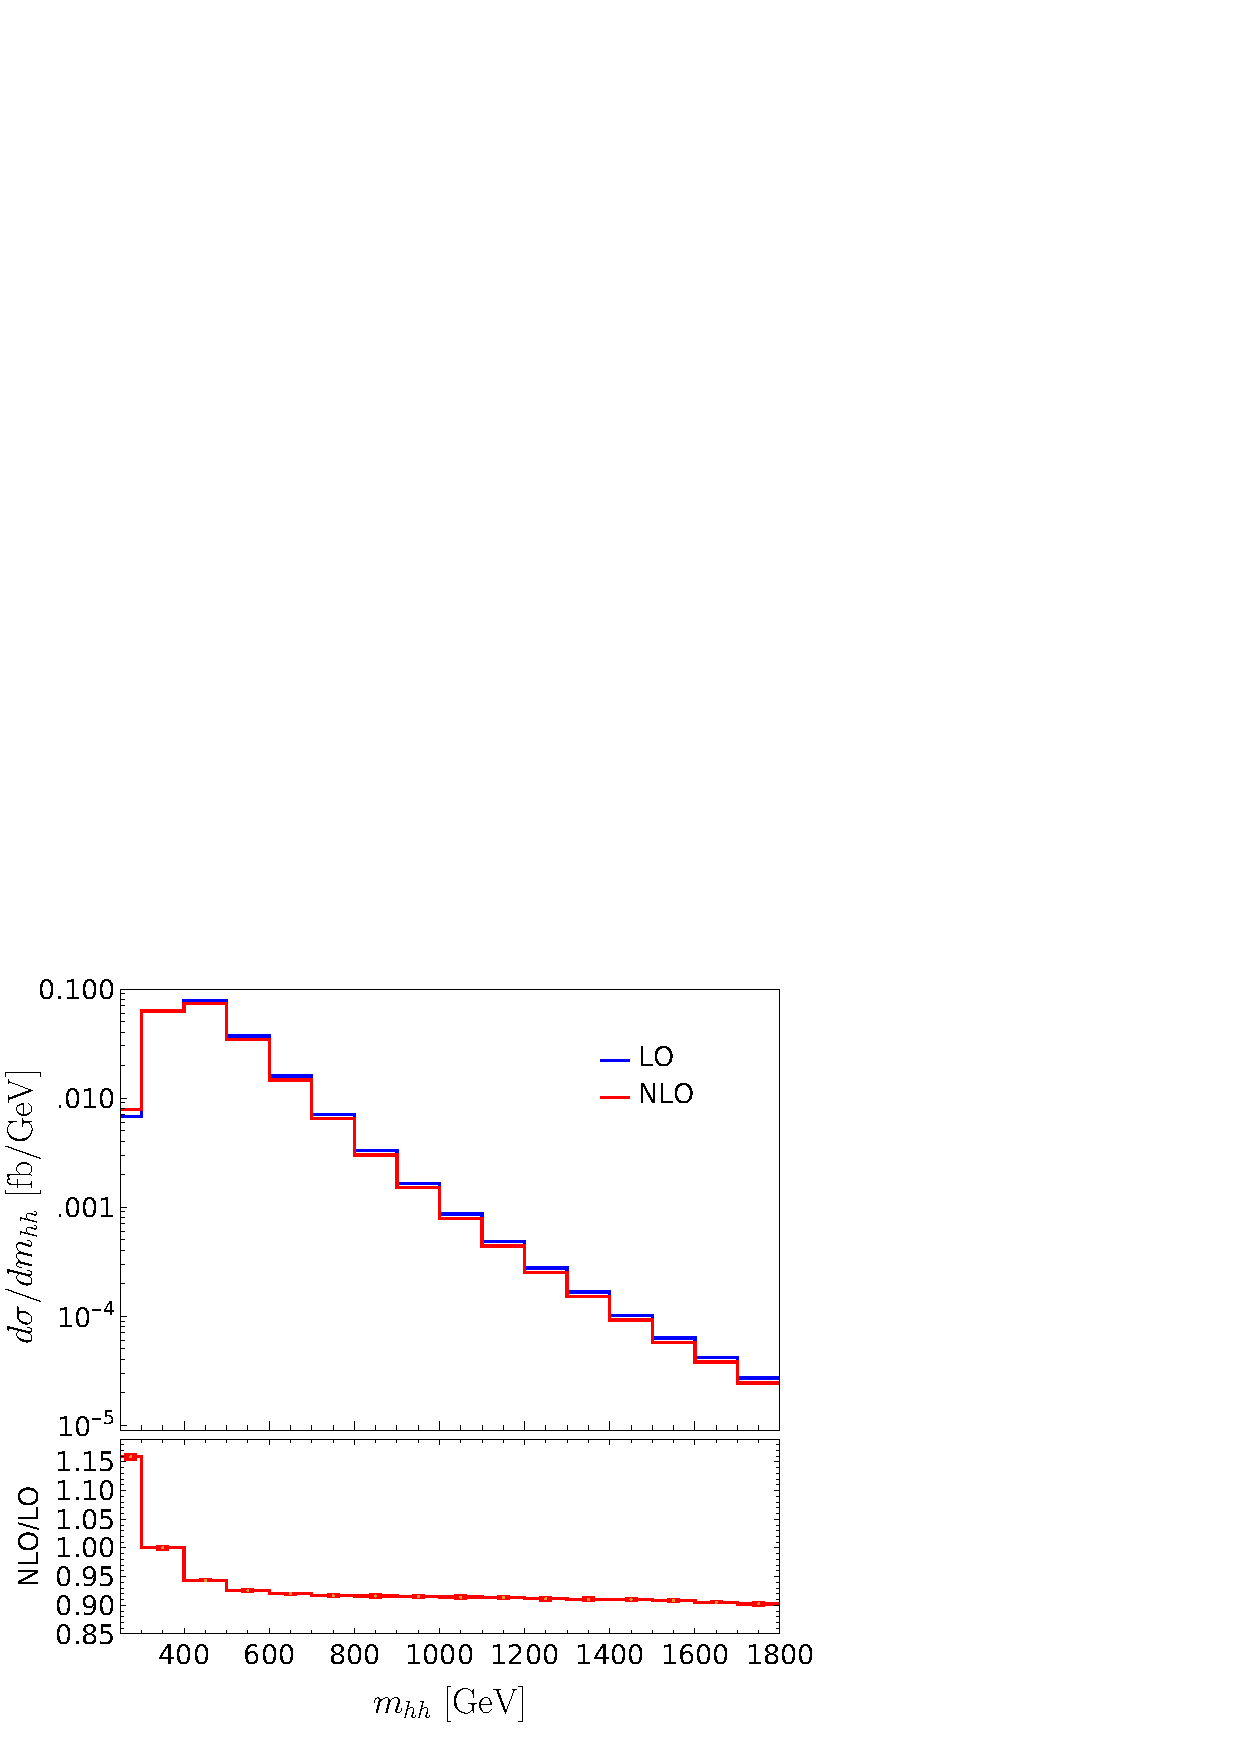
\includegraphics[width=0.47\textwidth]{NLO_EW_SM/EW_full/Images/NLO_FullEW_mhh_hlabels.pdf}}\label{mhh}}
    \subfloat[]{{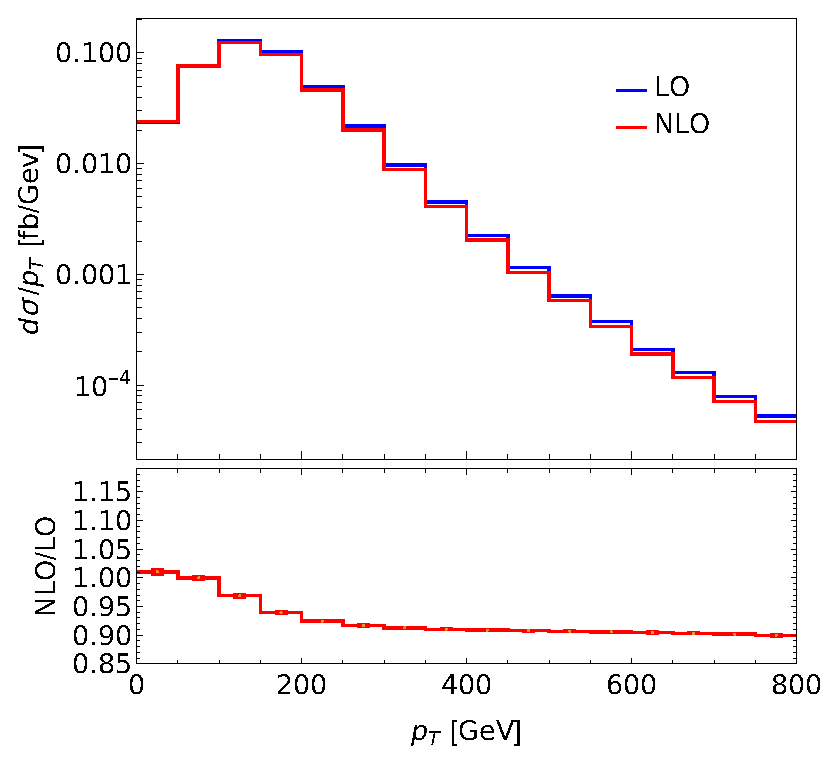
\includegraphics[width=0.47\textwidth]{NLO_EW_SM/EW_full/Images/NLO_FullEW_pth}}\label{pth}}
	\\
    \subfloat[]{{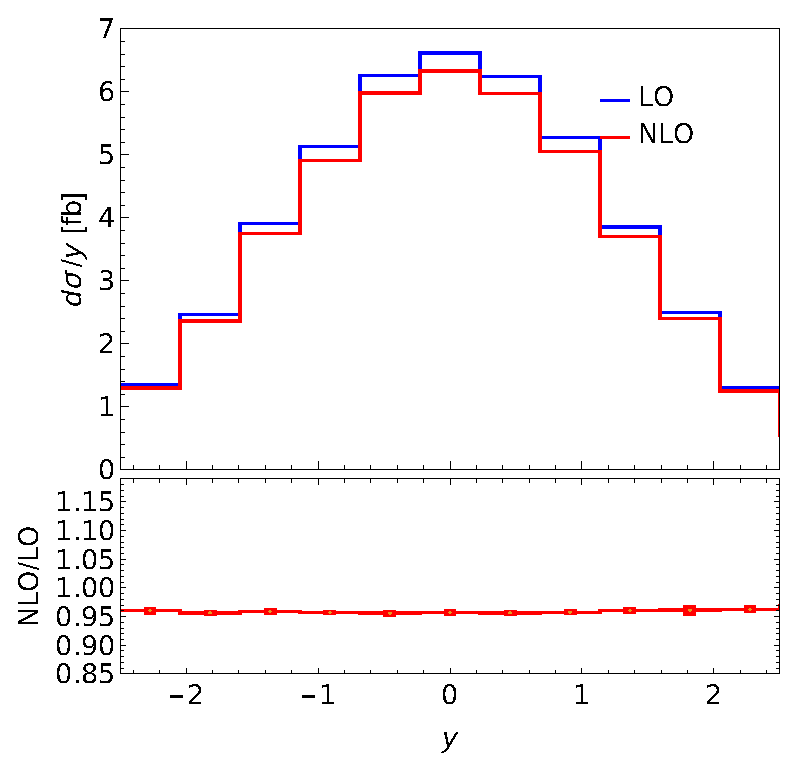
\includegraphics[width=0.47\textwidth]{NLO_EW_SM/EW_full/Images/NLO_FullEW_yh}}\label{yh}}
		\caption{Invariant mass distribution of the Higgs boson pair (a), transverse momentum distribution of one of the two Higgs bosons (b), and rapidity distribution of one of the two Higgs bosons (c), all at $\sqrt{s}=14\,\textup{TeV}$. In each panel, the upper plot shows absolute predictions and the lower panel displays the differential ${\cal K}$-factor with error bars representing statistical errors. Results shown are from Ref.~\cite{Bi:2023bnq}.}
    \label{fullEWobs}
\end{figure}


The invariant mass distribution of the Higgs boson pair $m_{hh}$ is shown in Fig.~\ref{mhh}. A significant positive correction, of approximately $+15\%$, is observed in the first bin. In fact, we find that the EW correction for phase space points near the $hh$ production threshold can exceed $+70\%$. As $m_{hh}$ increases, the $\mathcal{K}$ factor initially decreases dramatically and then becomes milder farther from the threshold. A similar pattern occurs for the $p_{T}$ distribution in Fig.~\ref{pth}, where the correction is initially positive before turning negative around $100\,\textup{GeV}$. For regions of large $m_{hh}$ or large $p_{T}$, the NLO EW correction is approximately $-10\%$. Note that, while the corrections can reach $-30\%$ for the squared matrix element at $\sqrt{\hat{s}} \approx 14\,\textup{TeV}$, the extreme suppression of the gluon luminosity at high energy makes this impact insignificant.

In Fig.~\ref{yh}, we display the rapidity distribution of one Higgs boson. The $\mathcal{K}$ factor is nearly flat, approximately $0.96$, matching that of the total cross section.



\FloatBarrier
\subsection{Breakdown of individual contributions}

\label{EW:breakdown}

Individual parts of the complete EW corrections to double Higgs boson production in gluon fusion have been computed separately, using a number of different methods.
Fig.~\ref{fig:bd} and Table~\ref{tab:bd} summarize the different contributions.


%\begin{figure}
%\centering
%    \subfloat[]{{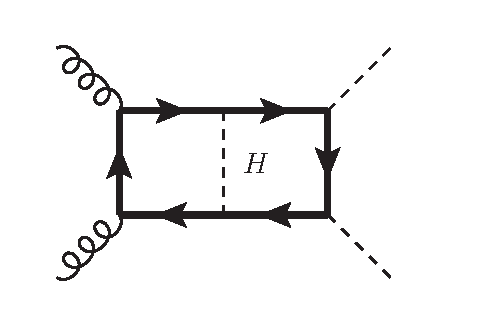
\includegraphics[width=0.3\textwidth]{EW_breakdown/Images/Yukawa}}}
%    \subfloat[]{{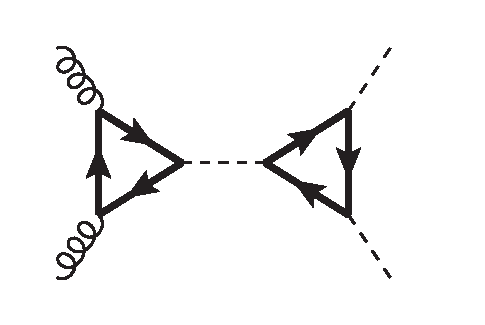
\includegraphics[width=0.3\textwidth]{EW_breakdown/Images/tt}}}
%    \subfloat[]{{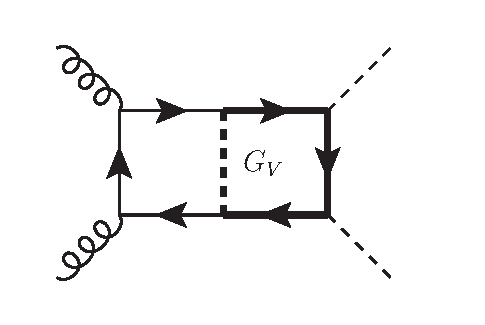
\includegraphics[width=0.3\textwidth]{EW_breakdown/Images/Goldstone}}}
%    \\[2em]
%    \subfloat[]{{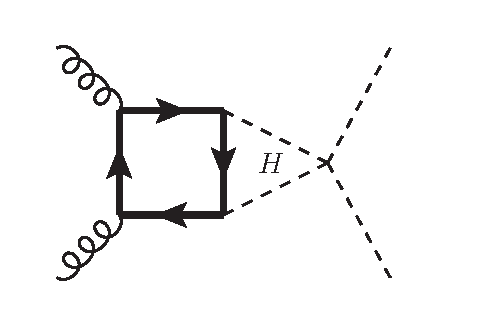
\includegraphics[width=0.3\textwidth]{EW_breakdown/Images/4H}}}
%    \subfloat[]{{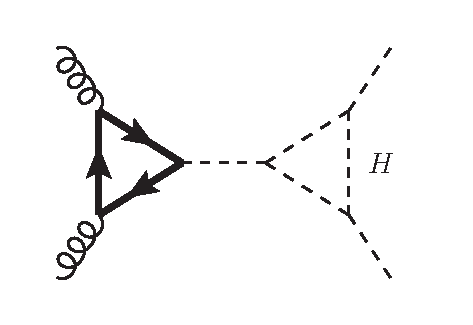
\includegraphics[width=0.3\textwidth]{EW_breakdown/Images/th}}}
%    \subfloat[]{{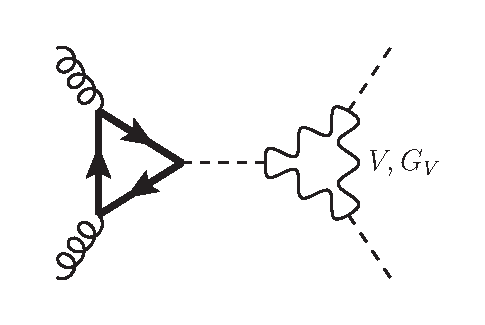
\includegraphics[width=0.3\textwidth]{EW_breakdown/Images/tv}}}
%    \\[2em]
%    \subfloat[]{{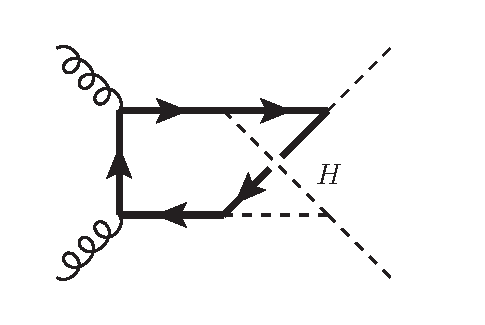
\includegraphics[width=0.3\textwidth]{EW_breakdown/Images/NP}}}
%    \subfloat[]{{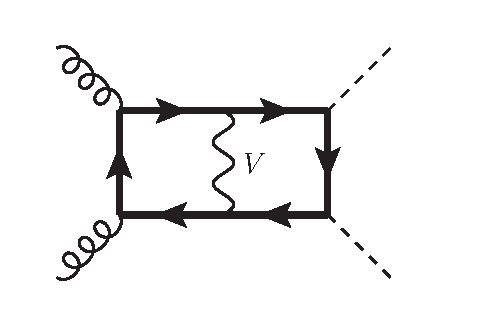
\includegraphics[width=0.3\textwidth]{EW_breakdown/Images/V}}}
%    \subfloat[]{{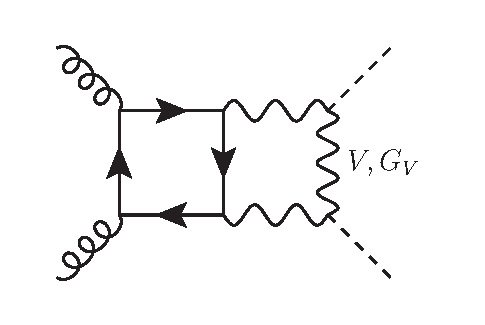
\includegraphics[width=0.3\textwidth]{EW_breakdown/Images/nl}}}
%\end{figure}


\begin{figure}
\centering
    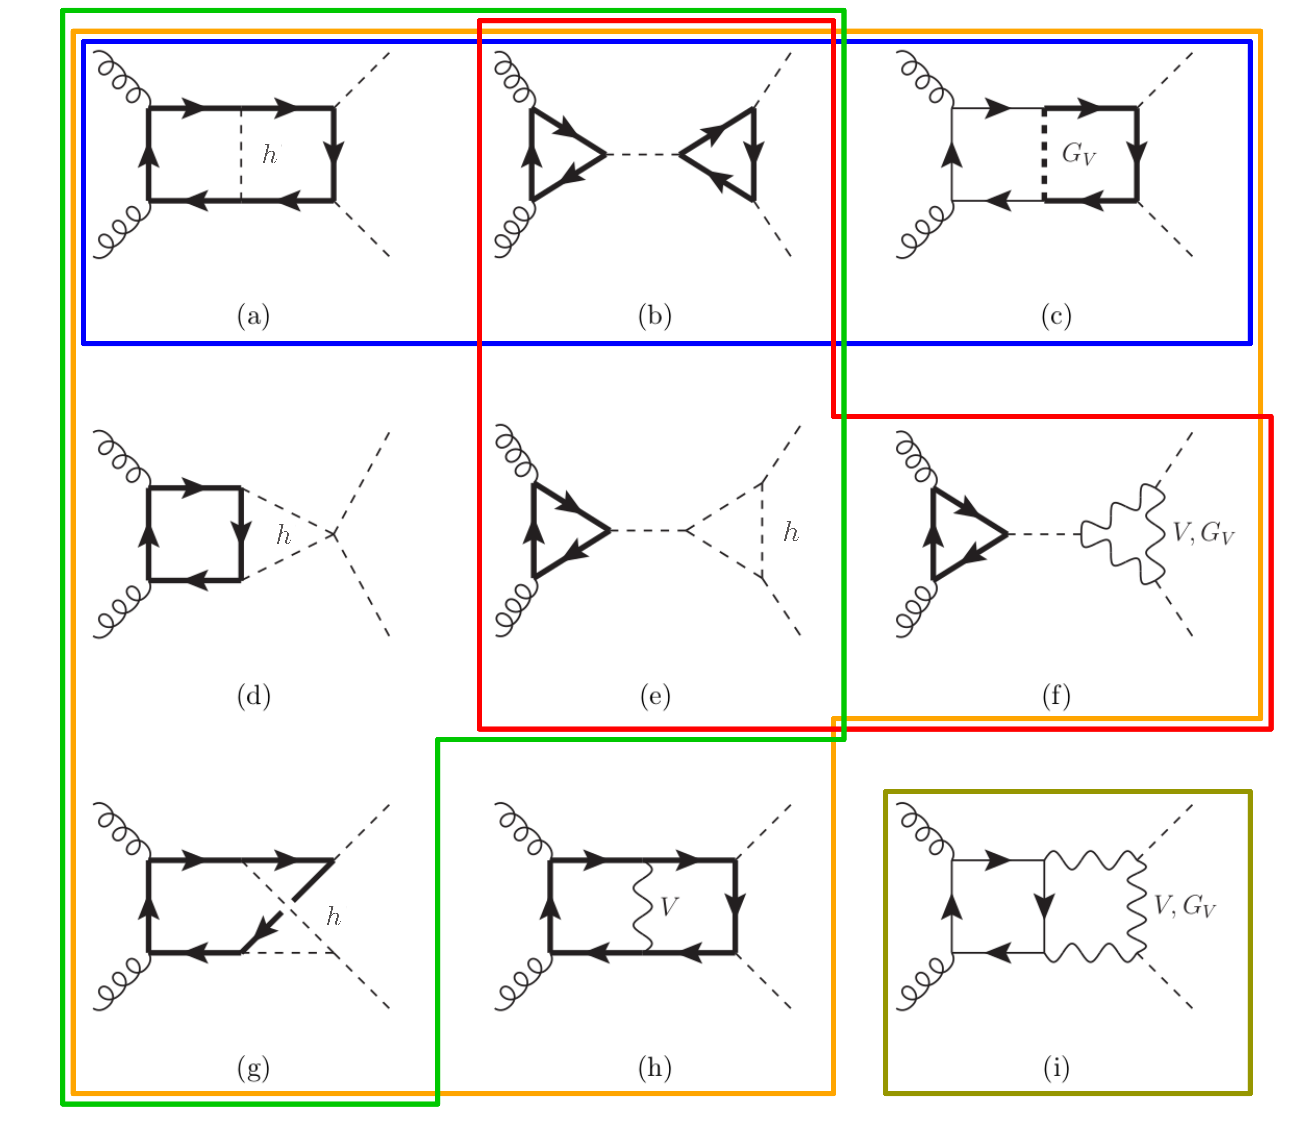
\includegraphics[width=\textwidth]{NLO_EW_SM/EW_breakdown/Images/blocks_hlabels.pdf}
	\caption{Example diagrams for different contributions. Blue set (a, b, c): top Yukawa-induced electroweak corrections; orange set (a, b, c, d, e, f, g, h): top quark contributions; red set (b, e, f): factorizable contributions; green set (a, b, d, e, g): top Yukawa and Higgs boson self-coupling corrections; olive set (i): light-quark contributions. The results of Section~\ref{EW:full} comprise all the displayed contributions. See Table~\ref{tab:bd}.}
    \label{fig:bd}
\end{figure}


\begin{table}
\begingroup
\small
\setlength{\tabcolsep}{2pt}
\begin{center}
\begin{tabularx}{\textwidth}{@{}
  >{\raggedright\arraybackslash}p{0.60\textwidth}
  c
  >{\raggedright\arraybackslash}X
@{}}
\toprule
Section & \mbox{Diagram sets} & \mbox{Key references} \\
\midrule
$\imineq{NLO_EW_SM/EW_breakdown/Images/BLUE}{1}$~Top Yukawa-induced electroweak corrections
  & (a), (b), (c)
  & \cite{Muhlleitner:2022ijf,Bhattacharya_TBA} \\

$\imineq{NLO_EW_SM/EW_breakdown/Images/ORANGE}{1}$~Top quark contributions
  & (a) to (h)
  & \cite{Davies:2023npk,Davies:2026wbx} \\

$\imineq{NLO_EW_SM/EW_breakdown/Images/RED}{1}$~Factorizable contributions
  & (b), (e), (f)
  & \cite{Muhlleitner:2022ijf,Zhang:2024rix} \\

$\imineq{NLO_EW_SM/EW_breakdown/Images/GREEN}{1}$~Top Yukawa and Higgs boson self-coupling corrections
  & (a), (b), (d), (e), (g)
  & \cite{Davies:2022ram,Davies:2025wke,Heinrich:2024dnz} \\

$\imineq{NLO_EW_SM/EW_breakdown/Images/OLIVE}{1}$~Light-quark contributions
  & (i)
  & \cite{Bonetti:2025vfd,Bhattacharya_TBA} \\
\bottomrule
\end{tabularx}
\caption{Breakdown of the individual EW contributions to $gg \to hh$ at two loops; see Fig.~\ref{fig:bd}. The results of Section~\ref{EW:full} correspond to the sum of all terms from (a) to (g).}
\label{tab:bd}
\end{center}
\endgroup
\end{table}

\subsubsection{Top Yukawa-induced electroweak corrections}

\label{EW:Top-Higgs_sector}

%\paragraph{Authors:}
%\begin{itemize}
%    \item Margarete Mühlleitner, Johannes Schlenk, Michael Spira~\cite{Muhlleitner:2022ijf};
%    \item Arunima Bhattacharya, Francisco Campanario, Sauro Carlotti, Jamie Chang, Javier Mazzitelli, Margarete Mühlleitner, Jonathan Ronca, Michael Spira ~\cite{Bhattacharya_TBA}.
%\end{itemize}

\noindent \textbf{Milada Margarete Mühlleitner, Johannes Schlenk, Michael Spira~\cite{Muhlleitner:2022ijf}.}

\noindent The first calculation of partial electroweak corrections to Higgs boson pair production via the dominant gluon-fusion process has been performed by investigating the corrections induced by the top Yukawa coupling \cite{Muhlleitner:2022ijf}. In order to set up a complete and consistent framework, these corrections have been obtained in the gaugeless limit, where all electroweak gauge couplings are set to zero, but the (massless) Goldstone contributions are taken into account, see Fig.~\ref{fig:bd}. This approach ensures the preservation of the $SU(2)$ symmetry of the scalar Higgs doublet. While the top-induced corrections to the trilinear Higgs boson self-coupling vertex are treated with the full top quark mass dependence, the triangle and box diagrams involving couplings of one or two Higgs bosons to gluons are treated in the HTL. The corresponding diagrams are displayed in Fig.~\ref{fg:dia_htl}, where the first two represent those that are treated in the HTL. For these two diagrams, we have used the effective Lagrangian \cite{Djouadi:1994ge,Muhlleitner:2022ijf}
\begin{equation}
{\cal L}_{eff} = \frac{\alpha_s}{12\pi} G^{a\mu\nu} G^a_{\mu\nu} \left\{
(1+\delta_1) \frac{H}{v} + ( 1 + \eta_1) \frac{H^2}{2v^2} + {\cal
O}(H^3) \right\}
\label{eq:leff}
\end{equation}
where
\begin{eqnarray}
\delta_1 & = & \frac{x_t}{2} + {\cal O}(x_t^2) \,, \qquad\qquad
\eta_1   = 4 x_t + {\cal O}(x_t^2) \,,
\label{eq:leff_coeff}
\end{eqnarray}
Here $x_t = G_F m_t^2/(8\sqrt{2}\pi^2)$, $G_F$ denotes the Fermi constant, $v$ is the vacuum expectation value (vev) of the Higgs field, and $m_t$ is the top quark mass. This effective Lagrangian describes the electroweak corrections induced by $x_t$ to the $hgg$ and $hhgg$ vertices in the HTL. We would like to point out explicitly that the square root of the wave-function counterterm of the external Higgs boson(s) is already taken into account in this effective Lagrangian.
\begin{figure}[!hbtp]
\centering
%\vspace*{-1.6cm}
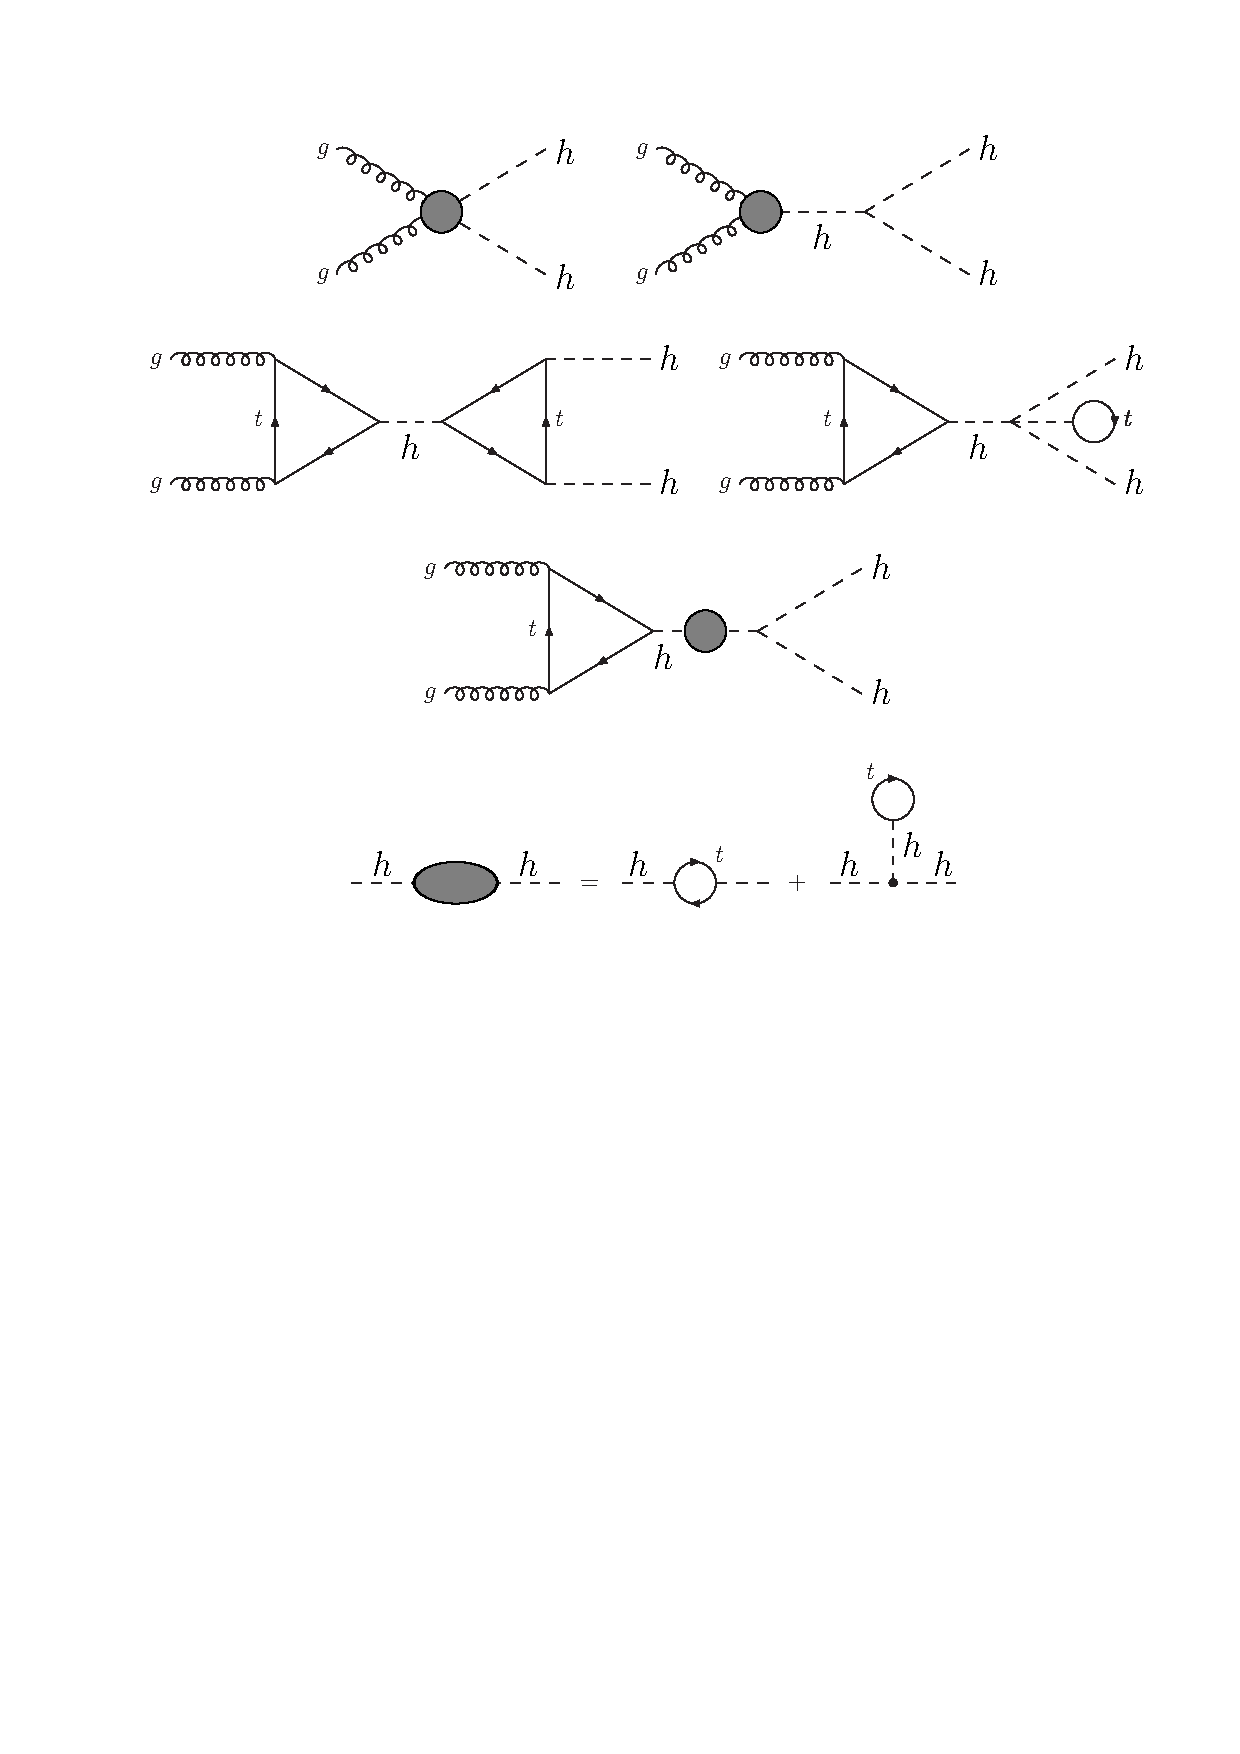
\includegraphics[width=0.9\textwidth]{NLO_EW_SM/EW_top-Higgs_sector/Images/dia_htl_hlabels.pdf}
%\vspace*{-8.3cm}
\caption{\label{fg:dia_htl}Generic diagrams contributing to the top Yukawa-induced electroweak corrections to the $gg\to hh$ process. The first two diagrams have been treated in the HTL. Diagrams adapted from Ref.~\cite{Muhlleitner:2022ijf}.}
\end{figure}
In Fig.~\ref{fg:dia_htl} the tadpole diagrams are displayed explicitly. We have used both the Fleischer--Jegerlehner scheme and the conventional scheme, in which the tadpole diagrams are omitted but retained in the corresponding counterterm of the trilinear Higgs boson self-coupling. We have obtained identical results in the final sum of the radiative corrections, once the vev $v$ is expressed in terms of the Fermi constant $G_F$.

Because the full top quark mass dependence of the one-loop times one-loop diagrams describing the radiatively corrected trilinear Higgs boson self-coupling vertex (all diagrams of Fig.~\ref{fg:dia_htl} except the first two) has been kept, the use of the effective trilinear Higgs boson self-coupling (derived from the effective Coleman--Weinberg potential \cite{Coleman:1973jx,Weinberg:1973ua,Jackiw:1974cv})
\begin{equation}
\lambda_{hhh} = 3 \frac{m_h^2}{v} \, , \qquad\qquad \lambda_{hhh}^{\rm eff} = \lambda_{hhh} - \frac{3 m_t^4}{\pi^2 v^3} \approx 0.91 \times \lambda_{hhh}
\end{equation}
to accommodate the dominant part of the radiative corrections can be tested. The result is that process-dependent, finite-momentum-dependent corrections are of the same size as the corrections above, growing with $m_t^4$,
\begin{eqnarray}
\sigma & = & K_{elw} \times \sigma_{LO} \nonumber \\
K_{elw} & \approx & 1.002 \hspace*{1.0cm} \mbox{($\lambda_{hhh}$)} \nonumber \\
K^{eff}_{elw} & \approx & 0.938 \hspace*{1cm} \mbox{($\lambda^{\rm eff}_{hhh}$)}.
\end{eqnarray}
Since the effective trilinear Higgs boson self-coupling generates about $6\%$ electroweak corrections to the total cross section artificially and larger corrections to the distributions, using the LO-like trilinear Higgs boson self-coupling $\lambda_{hhh}$ is favoured \cite{Muhlleitner:2022ijf}. The top Yukawa-induced electroweak corrections are small except in the region close to the production threshold due to the complete cancellation of the leading top quark mass terms in the LO matrix element, to which the corrections are normalized.

~

\noindent \textbf{Arunima Bhattacharya, Francisco Campanario, Sauro Carlotti, Jamie Chang, Javier Mazzitelli, Milada Margarete Mühlleitner, Jonathan Ronca, Michael Spira ~\cite{Bhattacharya_TBA}.}

\noindent The analysis of the top Yukawa-induced electroweak corrections discussed above has been extended to include the full top quark mass dependence. Specifically, the first two diagrams of Fig.~\ref{fg:dia_htl}, previously evaluated in the HTL, have been resolved into the corresponding two-loop diagrams involving top, bottom, Higgs, and Goldstone propagators. To preserve the SU(2) symmetry of the Higgs sector, this work has been performed in the gaugeless limit, enabling a gauge-invariant definition of the contributions associated with the top Yukawa coupling. In this limit, the Goldstone bosons are massless but do not generate infrared singularities. The method used for this calculation involves applying the projectors to the two form factors (in $D=4-2\epsilon$ dimensions), followed by a diagram-by-diagram Feynman parametrization. Since no tensor reduction has been used, the resulting Feynman integrands remain quite compact. The singularities were extracted by appropriate end-point subtractions. Moreover, this allowed us to keep, alongside the top quark mass, the bottom and the Higgs masses as free symbolic parameters. The virtual thresholds have been treated by introducing complex masses of the virtual propagators,
\begin{equation}
m_{t/b}^2 \to m_{t/b}^2 (1-i\bar\epsilon) \, , \qquad m_h^2 \to m_h^2 (1-i\bar\epsilon)
\end{equation}
with the regulator $\bar\epsilon$ to be sent to 0. The latter was achieved by applying a Richardson extrapolation \cite{Richardson} to a series of different values of $\bar\epsilon$. The minimal value of $\bar\epsilon$ used for numerical integrations varied between $10^{-8}$ and 0.1 depending on the diagram and the value of the invariant Higgs boson pair mass $Q=m_{hh}$. The top quark mass has been renormalized on-shell, and the vev has been renormalized according to the proper definition of the Fermi constant in muon decay.
\begin{figure}[!hbtp]
    \centering
    %\vspace*{-1.5cm}
    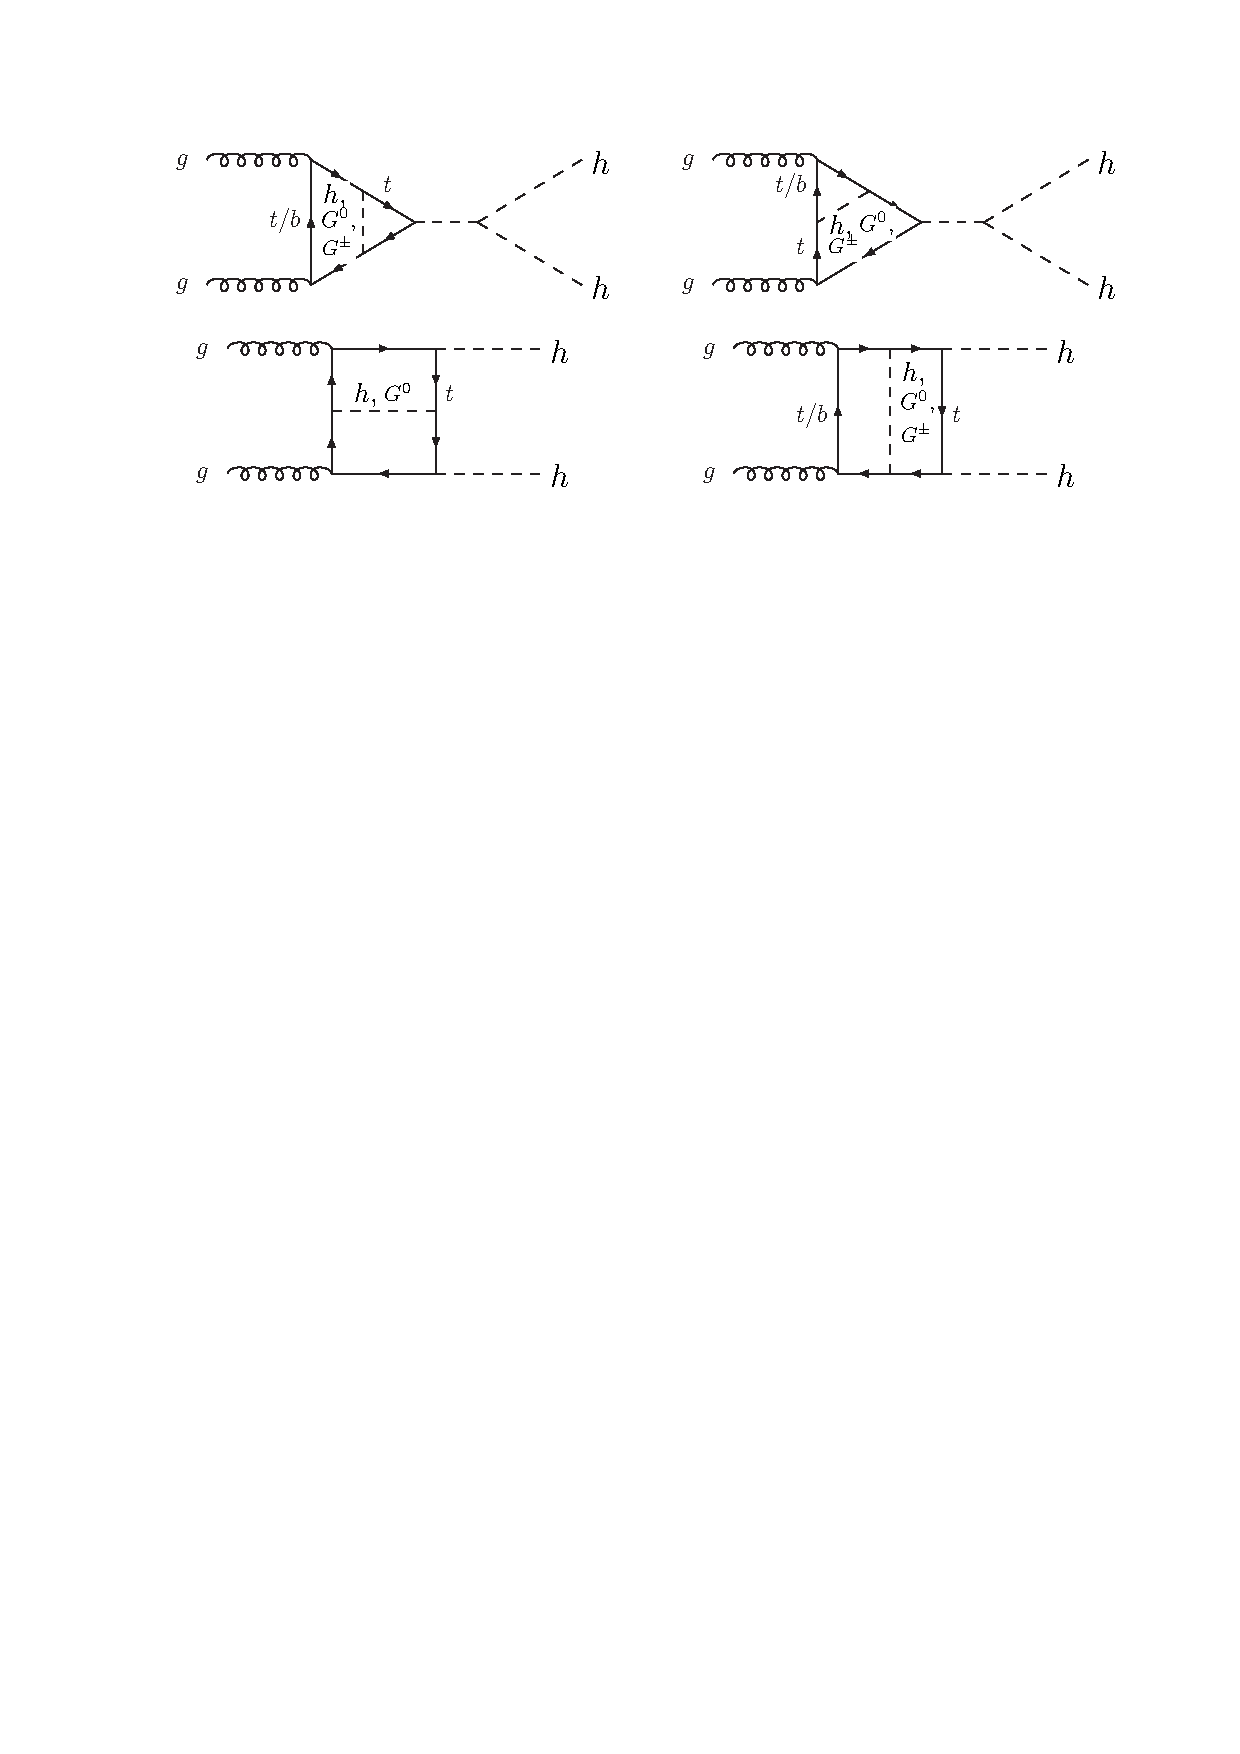
\includegraphics[width=0.8\textwidth]{NLO_EW_SM/EW_top-Higgs_sector/Images/dia_top_hlabels.pdf}
    %\vspace*{-13.9cm}
    \caption{\label{fg:dia_top}Sample two-loop triangle and box diagrams of the top Yukawa-induced electroweak corrections to Higgs boson pair production involving Higgs $h$ and Goldstone $G^0,G^\pm$ exchanges. The bottom propagators only contribute to the diagrams with charged Goldstone exchange. Diagrams from Ref.~\cite{Bhattacharya_TBA}.}
\end{figure}
\begin{figure}[!hbtp]
    \centering
    %\vspace*{-7cm}
    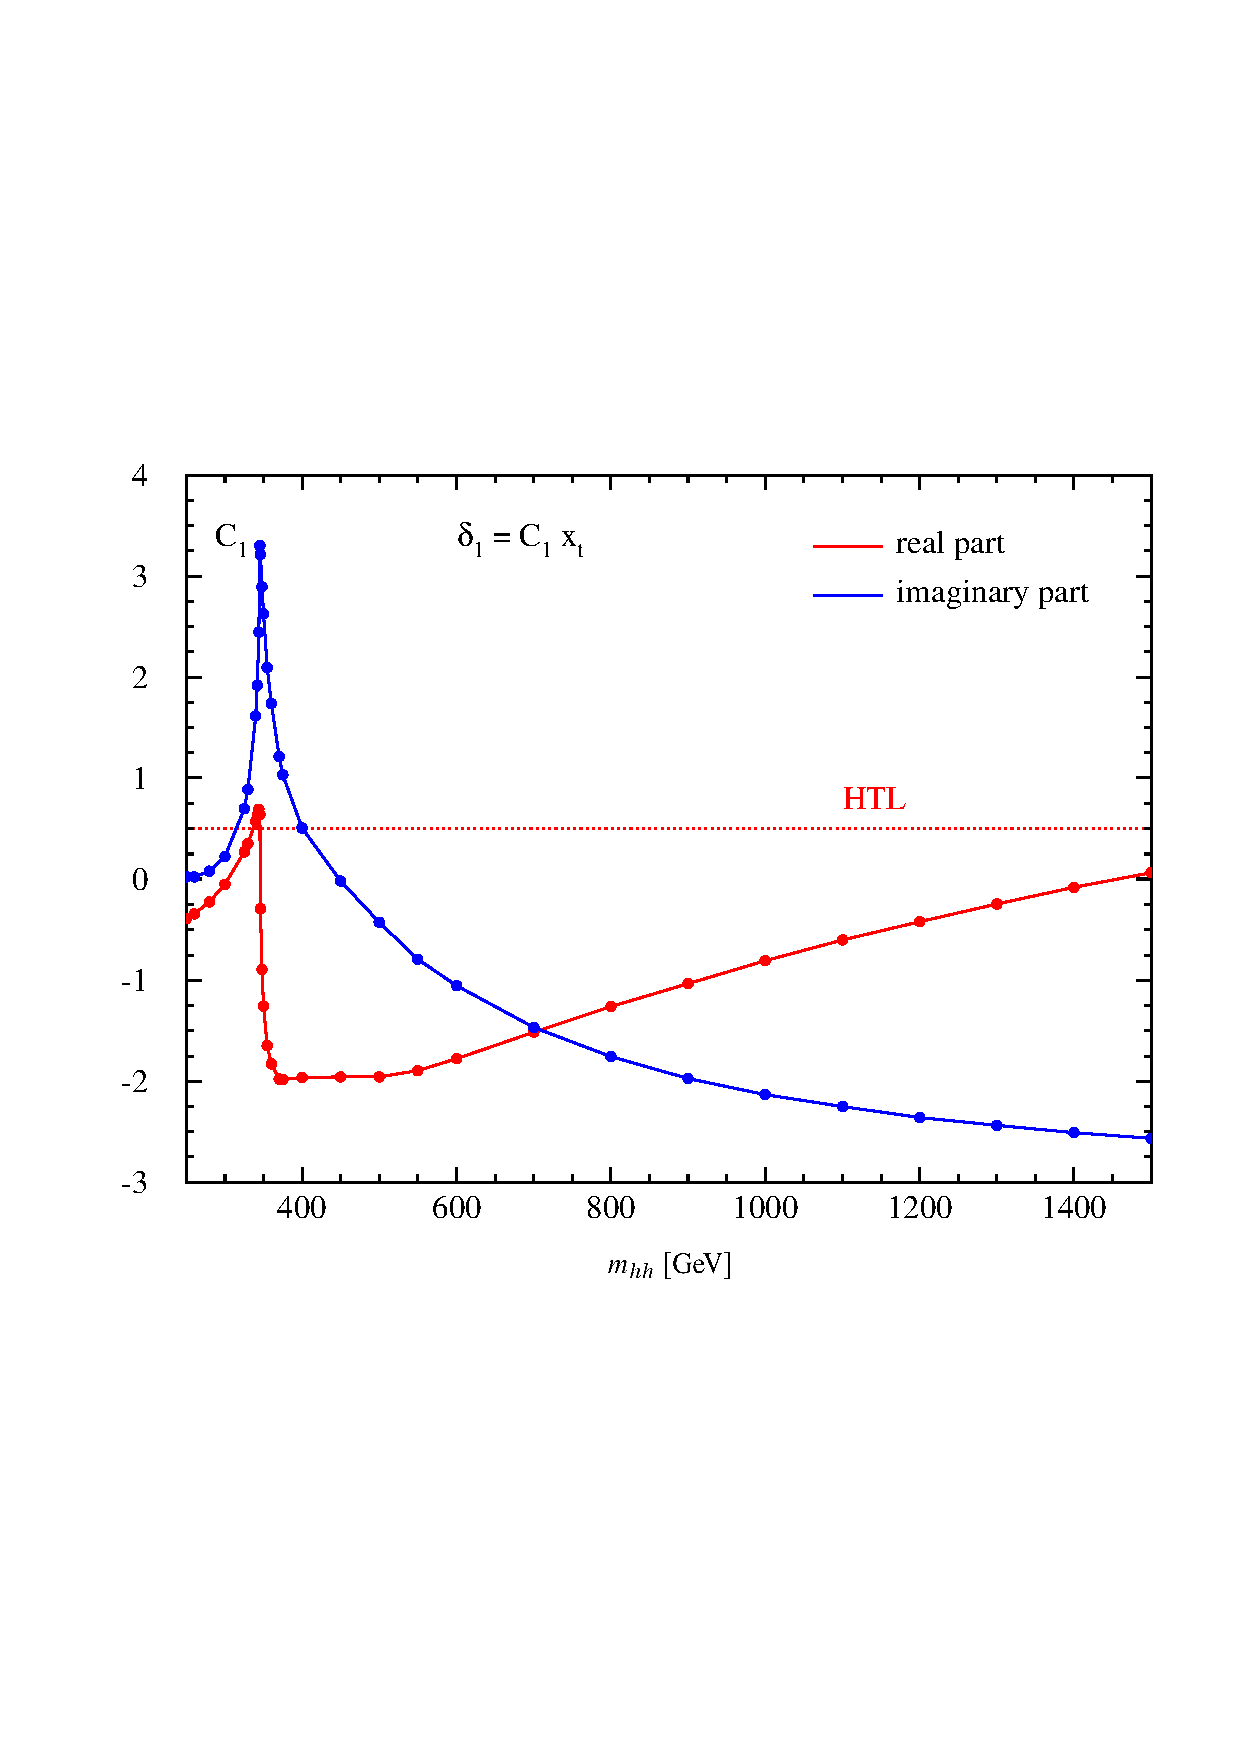
\includegraphics[width=0.7\textwidth]{NLO_EW_SM/EW_top-Higgs_sector/Images/d1tria_mhh.pdf}
    %\vspace*{-4.7cm}
    \caption{\label{fg:delta_1}The full top quark mass dependence of the coefficient $\delta_1$ of Eq.~\eqref{eq:leff_coeff} as a function of the invariant Higgs boson pair mass. The dotted line shows the purely real HTL result. The sizeable imaginary part arises from the diagrams with charged Goldstone exchange that include diagrams with $b\bar b$ thresholds. The points on the curve indicate the $m_{hh}$ values for which $\delta_1$ has been computed. The numerical errors are negligible and thus not shown. Results shown are from Ref.~\cite{Bhattacharya_TBA}.}
\end{figure}

The result of the two-loop triangle diagrams, see Fig.~\ref{fg:dia_top}, which can be directly compared to the coefficient $\delta_1$ in Eq.~\eqref{eq:leff_coeff}, is shown in Fig.~\ref{fg:delta_1}. As a cross-check, the HTL result of Eq.~\eqref{eq:leff_coeff} has been reproduced within uncertainties by artificially increasing the value of the top quark mass. The results indicate differences between the HTL and the full result at the (sub)percent level for the distribution in the Higgs boson pair mass.

The calculation of the two-loop box diagrams, see Fig.~\ref{fg:dia_top}, is more involved, since the additional phase space dependence does not allow for an immediate comparison with the HTL. Applying the same method as for the two-loop triangle diagrams and including the phase space integration in the numerical analysis, the result of the two-loop renormalized box diagrams plus the two-loop triangle diagrams and the previous one-loop times one-loop diagrams related to the radiative corrections to the trilinear Higgs boson self-coupling vertex is shown in Fig.~\ref{fg:del_top}, where the relative corrections are defined as
\begin{equation}
\sigma (gg\to hh) = \sigma_{LO} (gg\to hh)~( 1 + \delta_{\text{top Yukawa}} + \delta_{\text{light quarks}} )
\end{equation}
with the light-quark contributions $\delta_{\text{light quarks}}$ discussed in Section~\ref{EW:light-quark}. The total corrections are about $-5\%$ for intermediate values of $m_{hh}$ and are smaller for large values, while they are large close to the production threshold due to the large cancellation in the LO matrix element, to which the corrections are normalized. At large values of $m_{hh}$, the corrections develop a visible slope. The right panel of Fig.~\ref{fg:del_top} shows details of the $t\bar t$ threshold, which develops a sign-changing interference behaviour with the LO matrix element, with a maximum below the $t\bar t$ threshold.
\begin{figure}[!hbtp]
    \centering
    %\vspace*{-3.5cm}
%    \subfloat[]{{
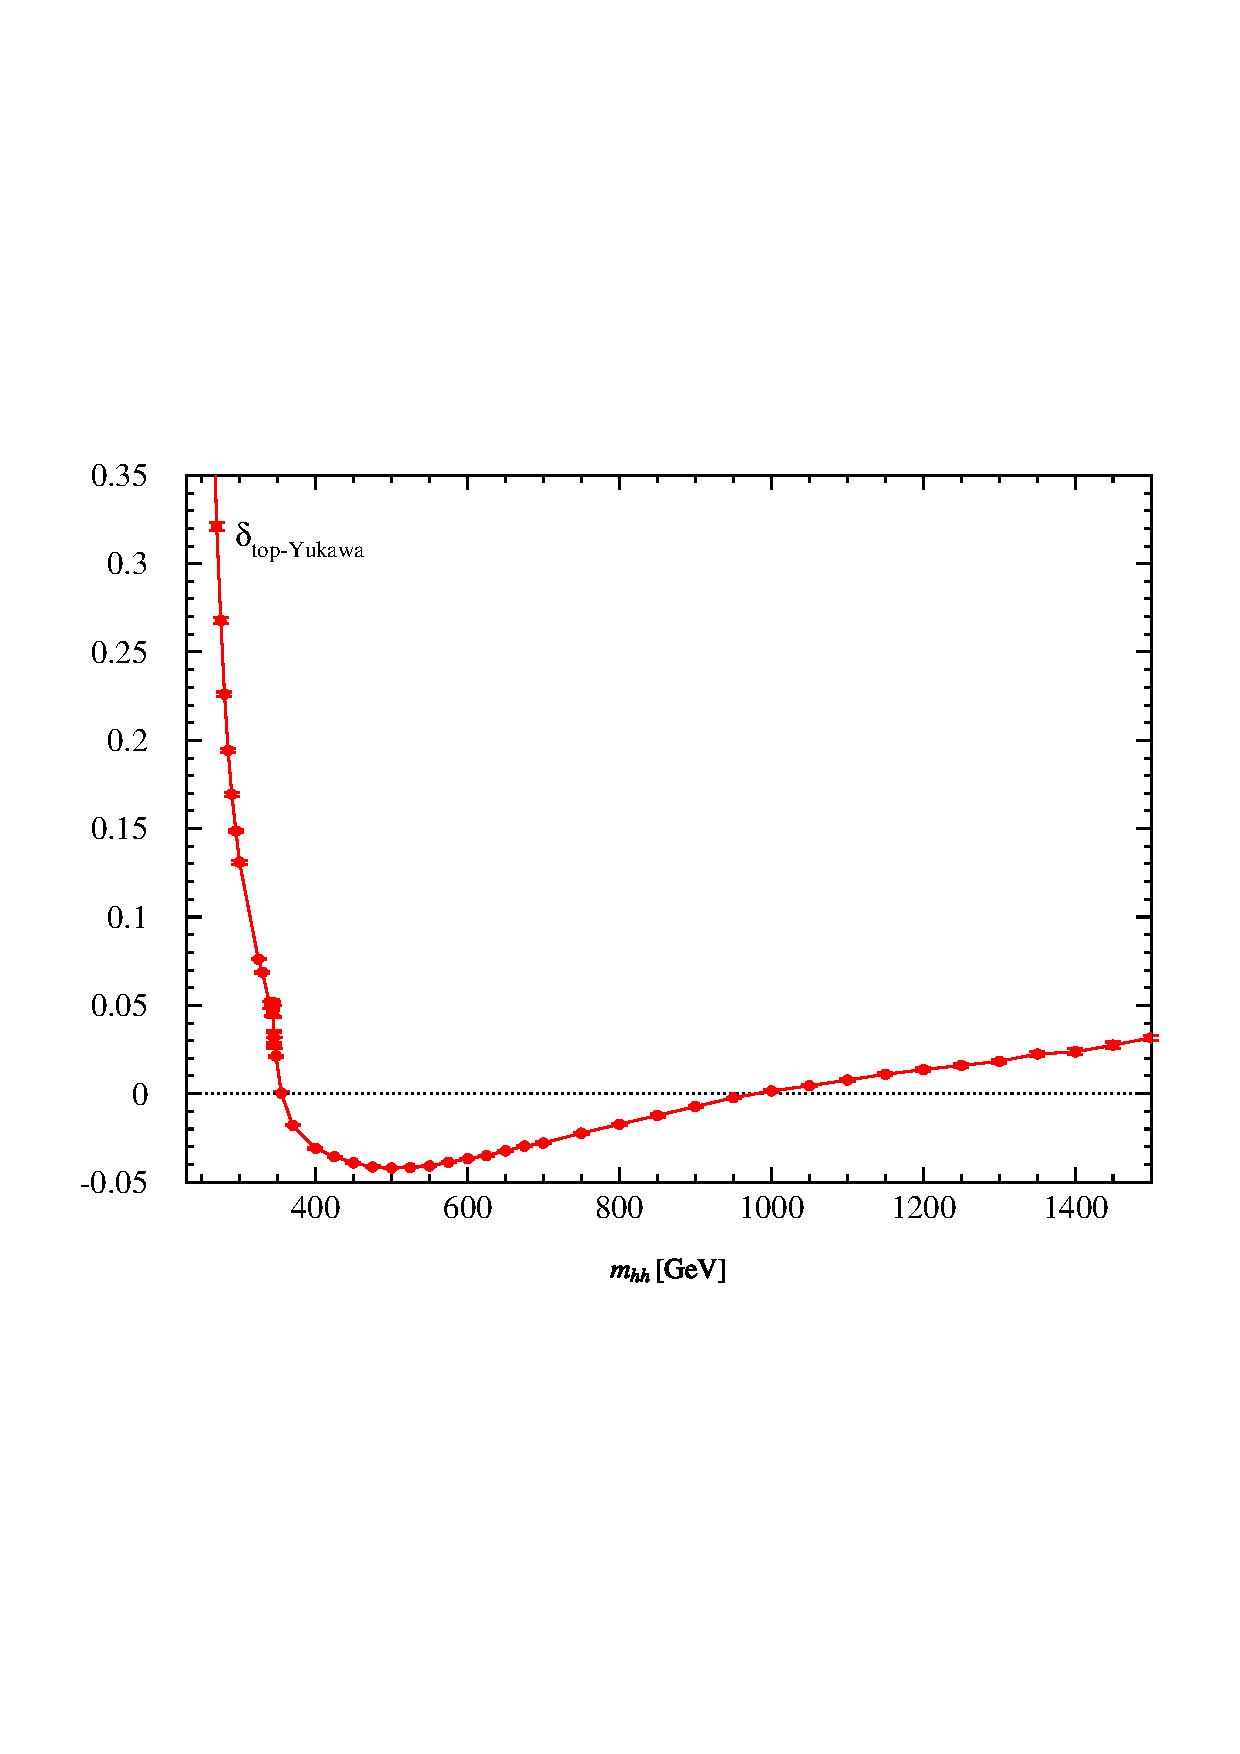
\includegraphics[width=0.49\textwidth]{NLO_EW_SM/EW_top-Higgs_sector/Images/del_top_mhh.pdf}
%}}
    %\vspace*{-10cm}
    %\%hspace*{-1.0cm}
%    \subfloat[]{{
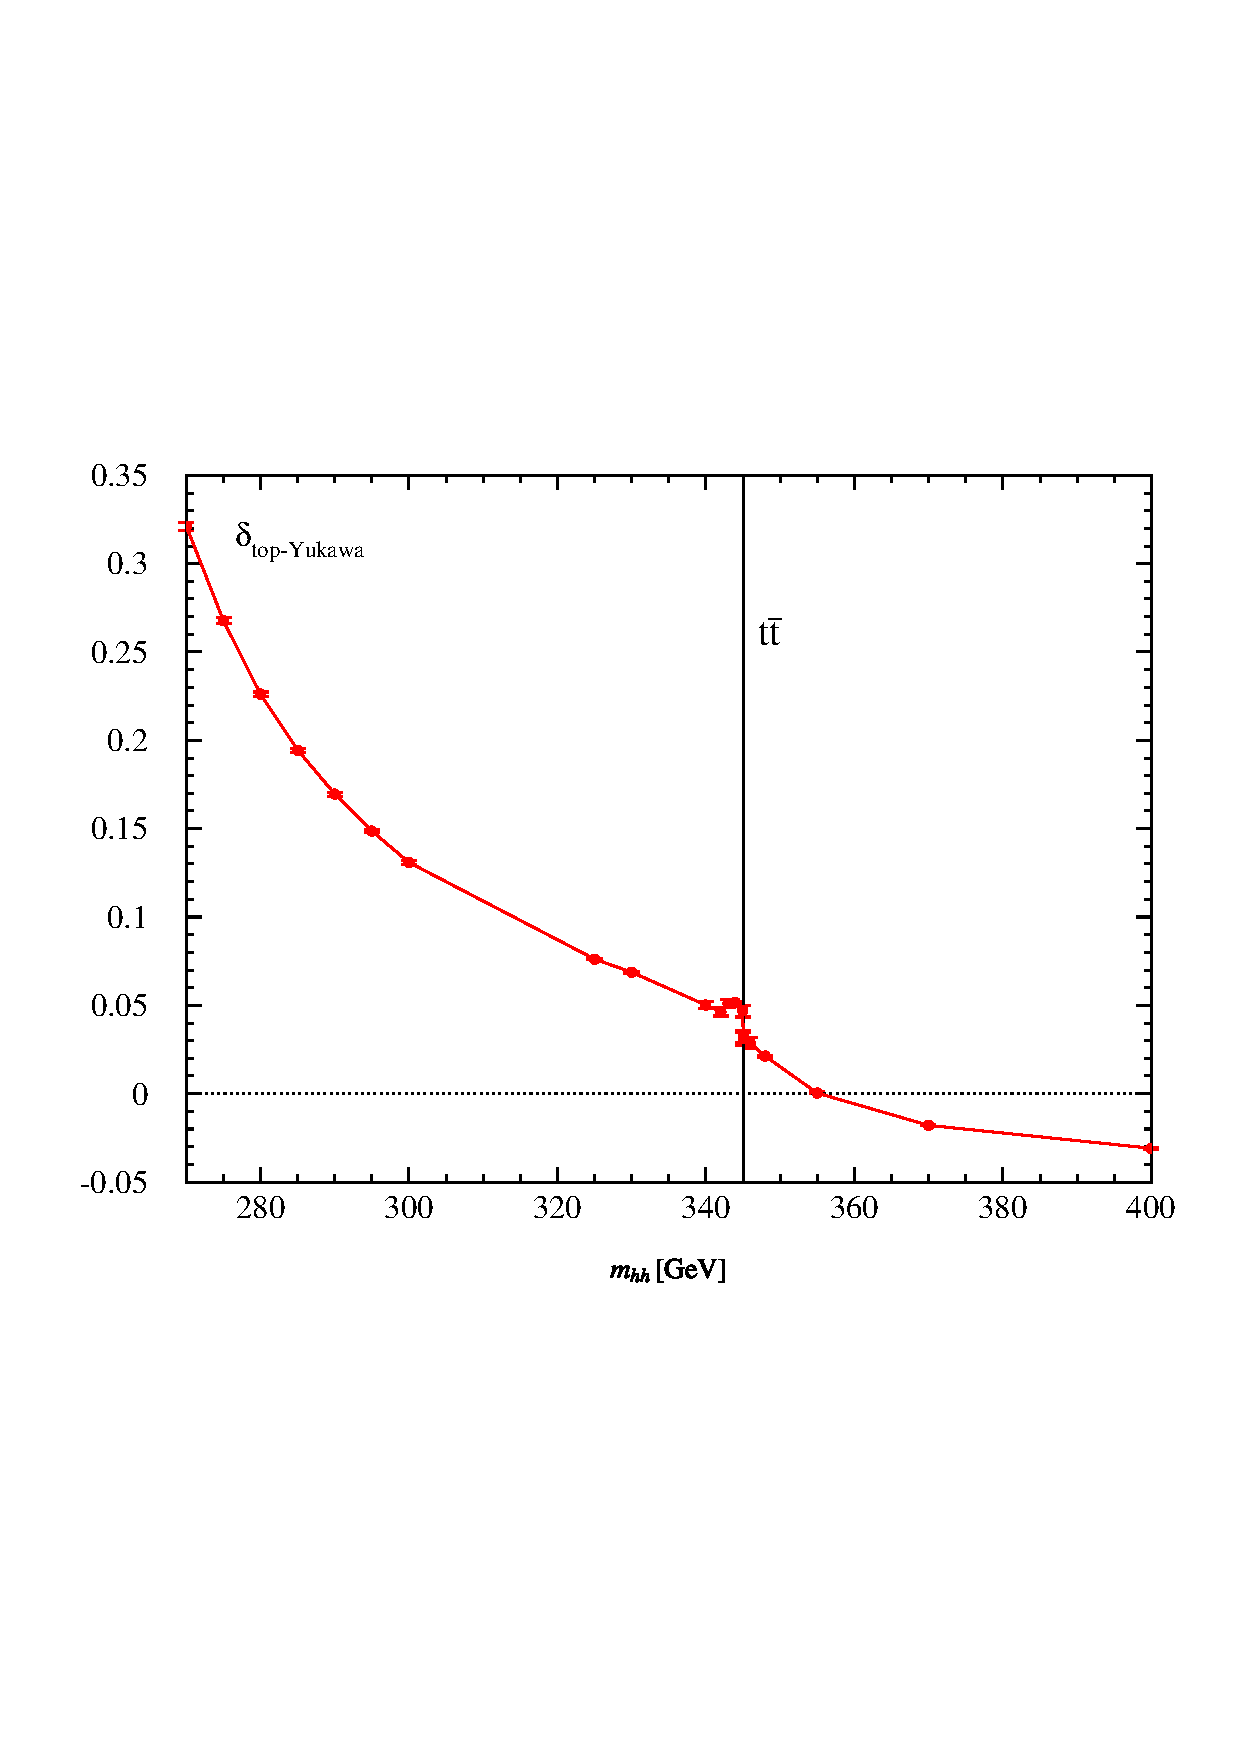
\includegraphics[width=0.49\textwidth]{NLO_EW_SM/EW_top-Higgs_sector/Images/del_top.detail_mhh.pdf}
%}}
    %\vspace*{6.0cm}
    \caption{The full relative top Yukawa-induced electroweak corrections to the $gg \to hh$ process. The points on the curve indicate the $m_{hh}$ values for which the corrections have been computed. The right panel shows a magnified view of the structure of the $t\bar t$ threshold. Numerical error bars are shown for each point. The vertical line indicates the position of the $t\bar t$ threshold. Results shown are from Ref.~\cite{Bhattacharya_TBA}.}
    \label{fg:del_top}
\end{figure}


\subsubsection{Top quark contributions}

\label{EW:top}

\noindent \textbf{Joshua Davies, Kay Schönwald, Matthias Steinhauser, Hantian Zhang~\cite{Davies:2023npk,Davies:2026wbx}.}

\noindent The full top quark contributions, including all sectors of the SM, have been computed analytically in
Refs.~\cite{Davies:2023npk,Davies:2026wbx} in the inverse top quark mass expansion and the high-energy expansion.

In the large-$m_t$ limit~\cite{Davies:2023npk}, expansions up to order $1/m_t^{10}$ have been computed in the Feynman gauge in the limit
\begin{align}
m_t^2 \, \gg \, s, \, |t|, \, m_h^2, \, m_W^2 , \, m_Z^2 \,,
\end{align}
where no additional hierarchy is assumed among the scales on the right-hand side.
%
The calculation has been analytically validated in the general $R_\xi$-gauge by assuming the hierarchy
\begin{align}
    m_t^2 \, \gg \, \xi_W \, m_W^2, \, \xi_Z \, m_Z^2  \, \gg \, s, \, |t|, \, m_h^2, \, m_W^2 , \, m_Z^2 \,,
\end{align}
where $\xi_W, \xi_Z$ are gauge parameters for the $W$ and $Z$ bosons.
%
These parameters appear in combination with gauge boson masses in the gauge boson and Goldstone propagators.
%
It is a valuable and non-trivial analytic validation that $\xi_W$ and $\xi_Z$ drop out in the renormalized amplitudes. 
%
Note that the gauge parameter for the photon, $\xi_\gamma$, drops out after summing all bare two-loop diagrams.
%


In the high-energy limit~\cite{Davies:2026wbx},
the electroweak calculation is much more challenging compared to the QCD case and the large-$m_t$ EW case. In this limit, we perform nested expansions in several small parameters in the following hierarchies in the Feynman gauge:
\begin{align}
    s, \, |t| \,  \gg \, m_t^2, \, m_W^2, \, m_Z^2 \,, (m_h^{\rm int})^2 \, \gg \,  (m_h^{\rm ext})^2\,,
\end{align}
where $m_h^{\rm int}$ denotes the mass of Higgs propagators inside the loop and $m_h^{\rm ext}$ is the mass of the final-state Higgs boson.
%
By identifying these hierarchies, we can first perform an external Higgs mass expansion, followed by expansions in the mass differences among several internal mass parameters as $\delta_X = 1 - m_X/ m_t $ for $ X=W,Z,H$.
Finally and most importantly, we perform a deep high-energy expansion with more than 100 expansion terms around the small-$m_t$ limit.
%
Schematically, the generic structure of the high-energy expansion of the form factors can be written as
\begin{align}
  F &= \sum_{n=-4}^{108} \sum_{i=0}^{2} \sum_{k_W=0}^{{4}}\sum_{k_Z=0}^{{4}}\sum_{k_H=0}^{{4}} 
        c_{ni}^{k_W k_Z k_H}  \: m_t^{n} \:
        (m^{\rm ext}_H)^{2i} \:
        \delta_W^{k_W} \: \delta_Z^{k_Z} \: \delta_H^{k_H} 
        \,,
\end{align}
where $c_{ni}^{k_W k_Z k_H}$ are coefficient functions of $s,t$ and $\log(m_t^2)$, featuring polylogarithmic and elliptic structures.
%
These analytic expressions are numerically evaluated through a Pad\'{e} procedure to increase the radius of convergence of the high-energy expansion across a larger phase space region.
%
The high-energy computation is technically challenging at both the form factor and Feynman integral level, due to drastically increased complexity when the full electroweak sector is taken into account.
%
We have successfully tackled both complexities and achieved a deep high-energy expansion up to the orders $m_t^{108}$, $(m_{H}^{\rm ext})^4$ and $\delta_X^4$. 
We have systematically analysed the convergence properties of our expansion, and we estimate the truncation uncertainty, dominated by the mass-difference expansion, to be about $\pm 1\%$ of the two-loop corrections.
%
For technical details of master integral calculations for the electroweak topologies, we refer to Refs.~\cite{Davies:2025wke,Davies:2022ram,Zhang:2024fcu}.



%%%
The electroweak renormalization follows the standard procedure as outlined in Refs.~\cite{Denner:1991kt,Denner:2019vbn}. 
%
The one-loop form factors are expressed in terms of parameters $\{e,m_W,m_Z,m_t,m_h\}$, and the parameter renormalization is performed with corresponding renormalization constants in the on-shell scheme.
%
The wave functions of the external Higgs bosons are also renormalized in the on-shell scheme.
%
Throughout the entire calculation, all tadpole contributions are consistently included such that all parameter renormalization constants are gauge-parameter independent, while the gauge-parameter dependence only appears in the wave function renormalization constant for the external Higgs boson.
%
This prescription is equivalent to the so-called \textit{Fleischer--Jegerlehner tadpole scheme}~\cite{Fleischer:1980ub}.
%

%%%%
The large-$m_t$ result~\cite{Davies:2023npk} supports the findings of Ref.~\cite{Muhlleitner:2022ijf},
where the top Yukawa-induced effects have been studied, namely that the electroweak corrections near the Higgs boson pair production threshold can lead to a few tens of percent effects with respect to the leading order contribution.
%
This interesting phenomenon is due to the fact that the electroweak corrections lift the destructive interference near the production threshold, where the matrix element is suppressed by the cancellation between triangle and box form factors at leading order.
Similarly, large top Yukawa-induced corrections near the production threshold have been found in Ref.~\cite{Heinrich:2024dnz}.
%
Although the radius of convergence is
limited, this result also serves as an important benchmark for other calculations. 
For example, it has been compared with Ref.~\cite{Bi:2023bnq} in a large-$m_t$ limit and good agreement was observed.

%
The high-energy result~\cite{Davies:2026wbx} has several interesting features.
In the limiting case of $m_h = 0$ and $m_t \to 0$, the leading high-energy expansion starts at $(m_t^2/s)^0$ at two loops, while it only starts at $(m_t^2/s)^1$ at one loop.
%
At NLO EW in this limit, we observe a quadratic and cubic logarithm ($\alpha \log^2(m_t^2/s)$ and $\alpha \log^3(m_t^2/s)$) as the leading logarithmic contribution for the box contributions in form factors $F_1$ and $F_2$, respectively. Note that the triangle contributions are suppressed at high energies due to the $s$-channel Higgs propagator.
%
In Fig.~\ref{fig::rEW_HE}, we present our result in terms of a ``partonic $K$-factor'' $r_{EW} = \frac{\alpha}{\pi} \big( \, \mathcal{U}^{(0,1)} / \mathcal{U}^{(0)} \big)$ up to $\sqrt{s} = 10$~TeV, where we assume the perturbative NLO QCD and EW expansion as $|\mathcal{M}|^2 = \bar{X}_0 \big( \, \mathcal{U}^{(0)} + \frac{\alpha_s}{\pi}\, \mathcal{U}^{(1,0)} + \frac{\alpha}{\pi} \, \mathcal{U}^{(0,1)} \big)$ with an overall prefactor $\bar{X}_0$.
\begin{figure}[t]
\centering
    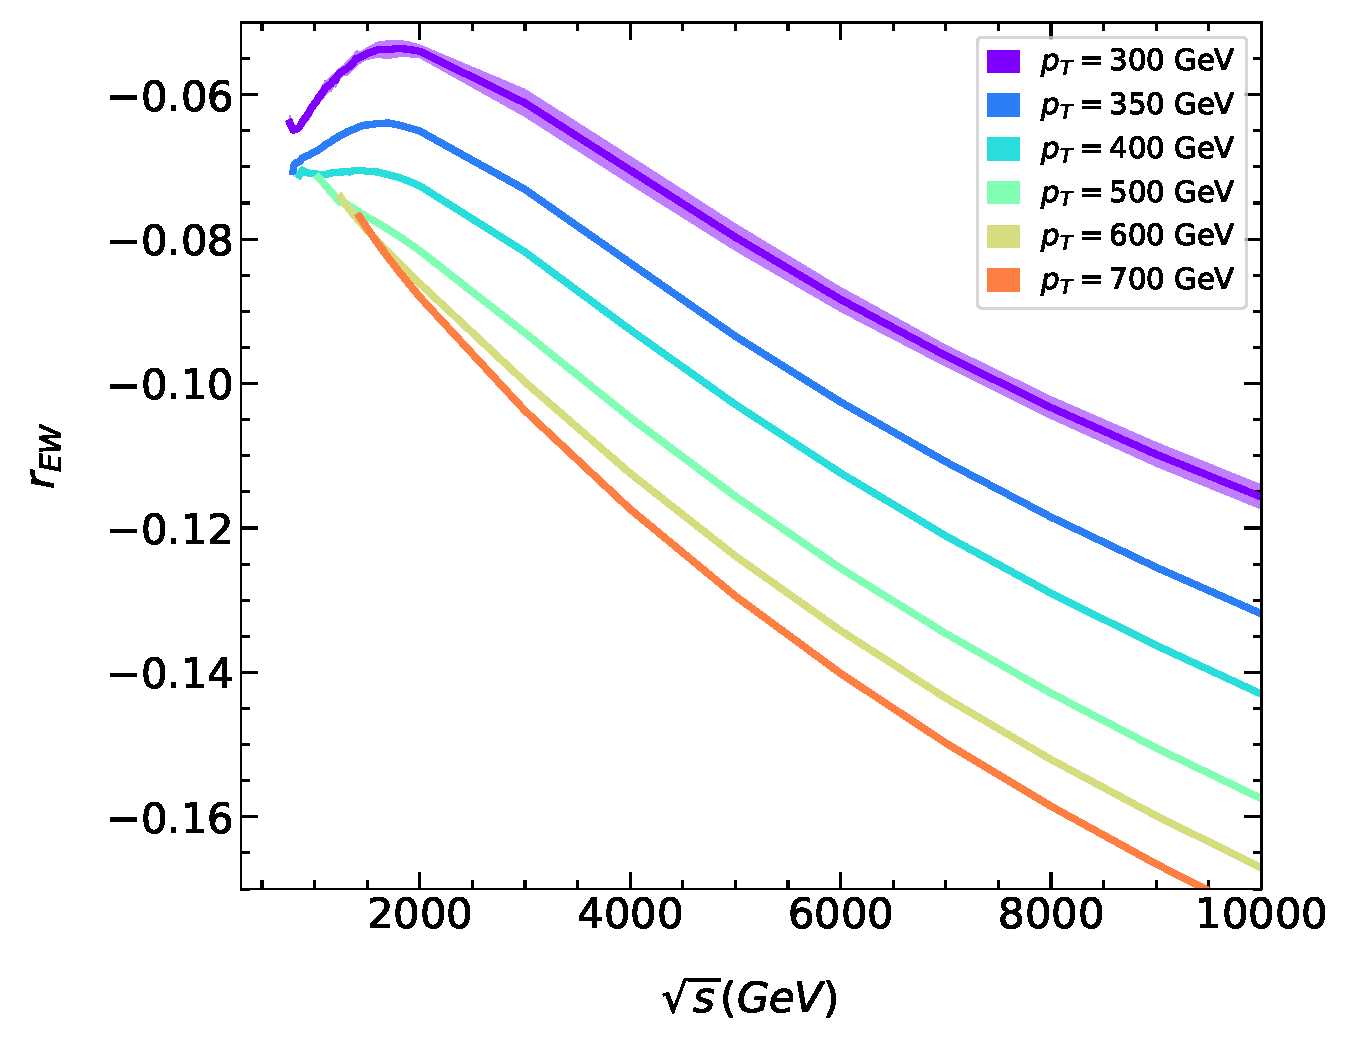
\includegraphics[width=.65\textwidth]{NLO_EW_SM/EW_top/figs/rEW_HE.pdf}
  \caption{\label{fig::rEW_HE}
   $r_{\rm EW}$ for various values of $p_T$ as a function of $\sqrt{s}$.
   The plots show the same data for different ranges of $\sqrt{s}$ on the $x$ axis. The uncertainty band (only visible for $p_T = 300$~GeV) is obtained from the Pad\'{e} approximation, and the truncation uncertainty in the $\delta_X$ and $m_h^{\rm ext}$ expansions is not shown but is estimated to be $\pm1\%$.
   Results shown are from Ref.~\cite{Davies:2026wbx}.
   }
\end{figure}
Our result covers a large phase space ranging from the high-energy limit to fairly low values of Higgs transverse momentum $p_T \gtrsim 350$~GeV.
It shows that these electroweak corrections lead to an effect of order $-10\%$, supporting the observation from Ref.~\cite{Bi:2023bnq} for the hadronic invariant mass or $p_T$ distribution.


\subsubsection{Factorizable contributions}

\label{EW:1loopX1loop}

%\paragraph{Authors:}
%\begin{itemize}
%    \item Margarete Mühlleitner, Johannes Schlenk, Michael Spira~\cite{Muhlleitner:2022ijf};
%    \item Joshua Davies, Kay Schönwald, Matthias Steinhauser, Hantian Zhang~\cite{Zhang:2024rix}.
%\end{itemize}


Factorizable contributions consist of diagrams containing two separated one-loop corrections, see Fig.~\ref{fig:bd}, cases (b), (e), and (f).


\noindent \textbf{Milada Margarete Mühlleitner, Johannes Schlenk, Michael Spira~\cite{Muhlleitner:2022ijf}.}

\noindent The subset of factorizable contributions containing Yukawa interactions between the Higgs and the top quark (case (b)) has been evaluated analytically retaining full dependence on masses and kinematics. Analytical results have been presented in Ref.~\cite{Muhlleitner:2022ijf}.


\noindent \textbf{Joshua Davies, Kay Schönwald, Matthias Steinhauser, Hantian Zhang~\cite{Zhang:2024rix}.}

\noindent Exact analytic results for the complete set of factorizable contributions in the SM have been obtained (cases (b), (e), and (f)). No approximation has been applied. Computer-readable results for the form factors are provided, expressed in terms of standard $B_0$ and $C_0$ functions.


\subsubsection{Top Yukawa and Higgs boson self-coupling corrections}

\label{EW:Top-Higgs_self}

%\paragraph{Authors:}
%\begin{itemize}
%    \item Joshua Davies, Kay Schönwald, Matthias Steinhauser, Hantian Zhang~\cite{Davies:2022ram,Davies:2025wke};
%    \item Gudrun Heinrich, Stephen Jones, Matthias Kerner, Thomas Stone, Augustin Vestner~\cite{Heinrich:2024dnz}.
%\end{itemize}


\noindent \textbf{Joshua Davies, Kay Schönwald, Matthias Steinhauser, Hantian Zhang~\cite{Davies:2022ram,Davies:2025wke}.}

\noindent Analytic high-energy results for the subset of Feynman diagrams involving top Yukawa and Higgs boson self-energy couplings have been computed in Refs.~\cite{Davies:2022ram,Davies:2025wke}.  Such diagrams involve as dimensionful quantities the Mandelstam variables $s$ and $t$, the top quark mass and the Higgs boson mass.  In the calculation the final-state Higgs mass and the one in the propagators inside the loop diagrams are treated separately. This allows us to perform as a first step an expansion in the final-state mass and subsequently an expansion in $\delta = 1-m_h^{\rm int}/m_t$ with $m_h^{\rm int}$ being the internal propagator mass. Both expansions are simple Taylor expansions.
Afterwards, we realize the high-energy limit through an expansion for small $m_t$ which requires the application of a nontrivial asymptotic expansion.
%
Technical details of the master integral calculations in the high-energy limit are given in Refs.~\cite{Zhang:2024fcu,Davies:2022ram,Davies:2025wke}, together with a publicly available tool \texttt{AsyInt}~\cite{Zhang:2024fcu}.
%
We typically compute about $100$ expansion terms in $m_t$ and subsequently apply a Pad\'e procedure that provides, for each phase-space point, a central value and an uncertainty. It has been shown in Refs.~\cite{Davies:2022ram, Davies:2023vmj} that this approach leads to precise results down to fairly low values of the Higgs transverse momentum $p_T$ in the case of QCD and leading Yukawa corrections.

As an illustration we show in Fig.~\ref{fig::diff_to_SD_yt3lam1} the comparison of the real part of the box contribution to form factor $F_1$ originating from diagrams with three top quark Yukawa couplings and one trilinear Higgs boson self-coupling (see Fig.~\ref{fig::diags} for sample diagrams) to the numerical results from Ref.~\cite{Heinrich:2024dnz}. After including expansion terms up to order $m_h^4\delta^3$ one observes agreement at the percent level.

Note that the analytic results provide full flexibility concerning the change of renormalization schemes and the variation of input parameters.

\begin{figure}
\centering
    \subfloat[]{{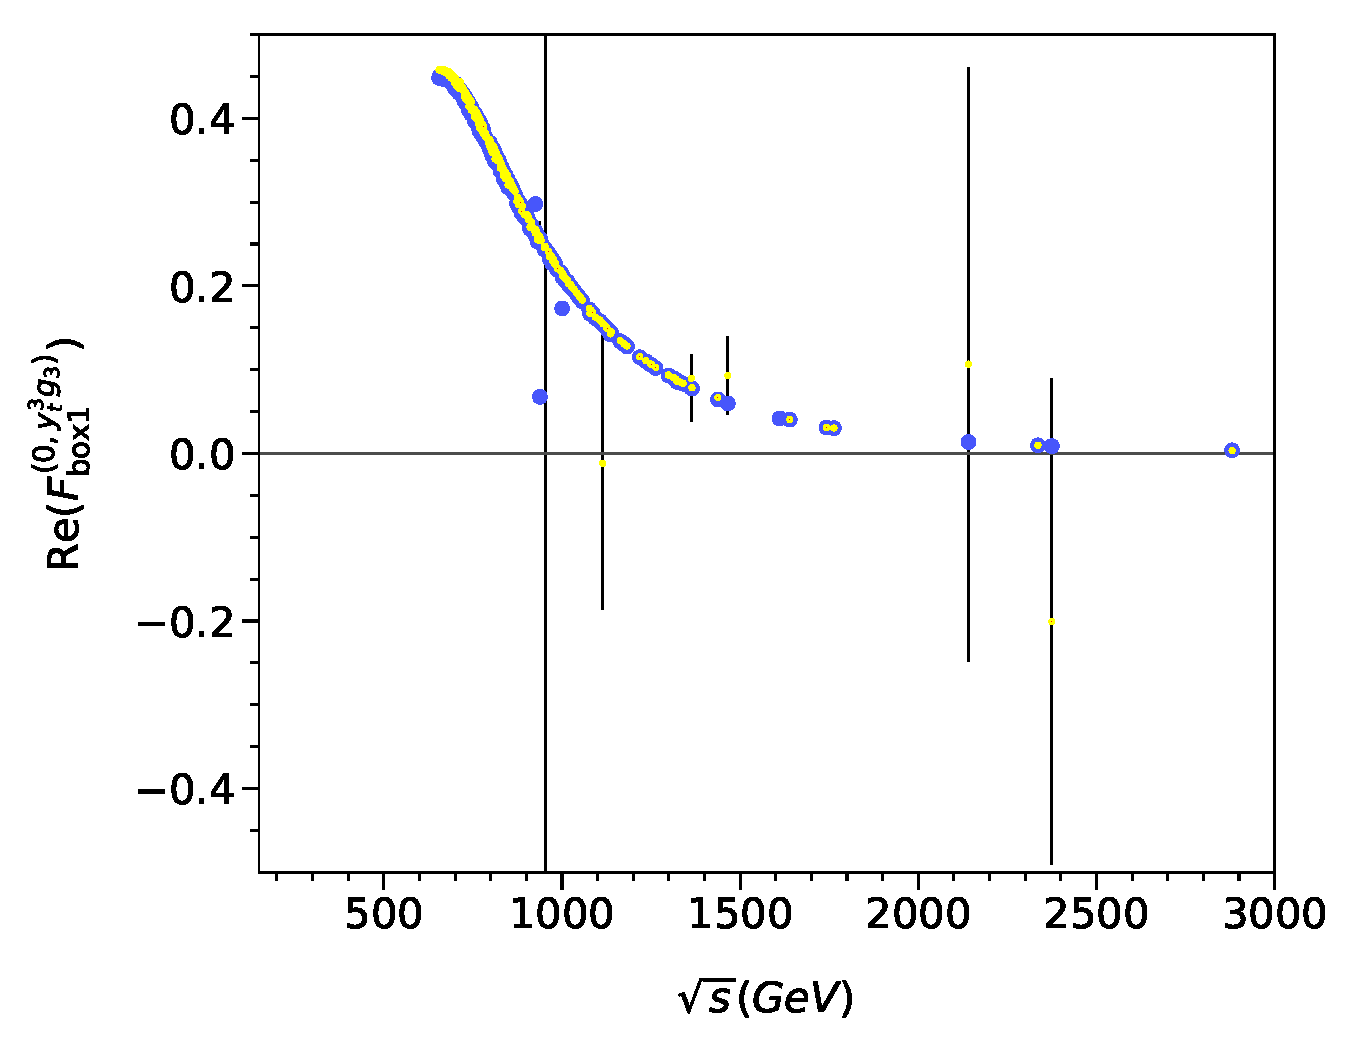
\includegraphics[width=0.48\textwidth]{NLO_EW_SM/EW_top-Higgs_self/Images/diff_to_SD_F1bare_ep0_t-plus_mhs2del3_yt3lam1_pTcut300_re_sqrts_FF}}}
	\\
    \subfloat[]{{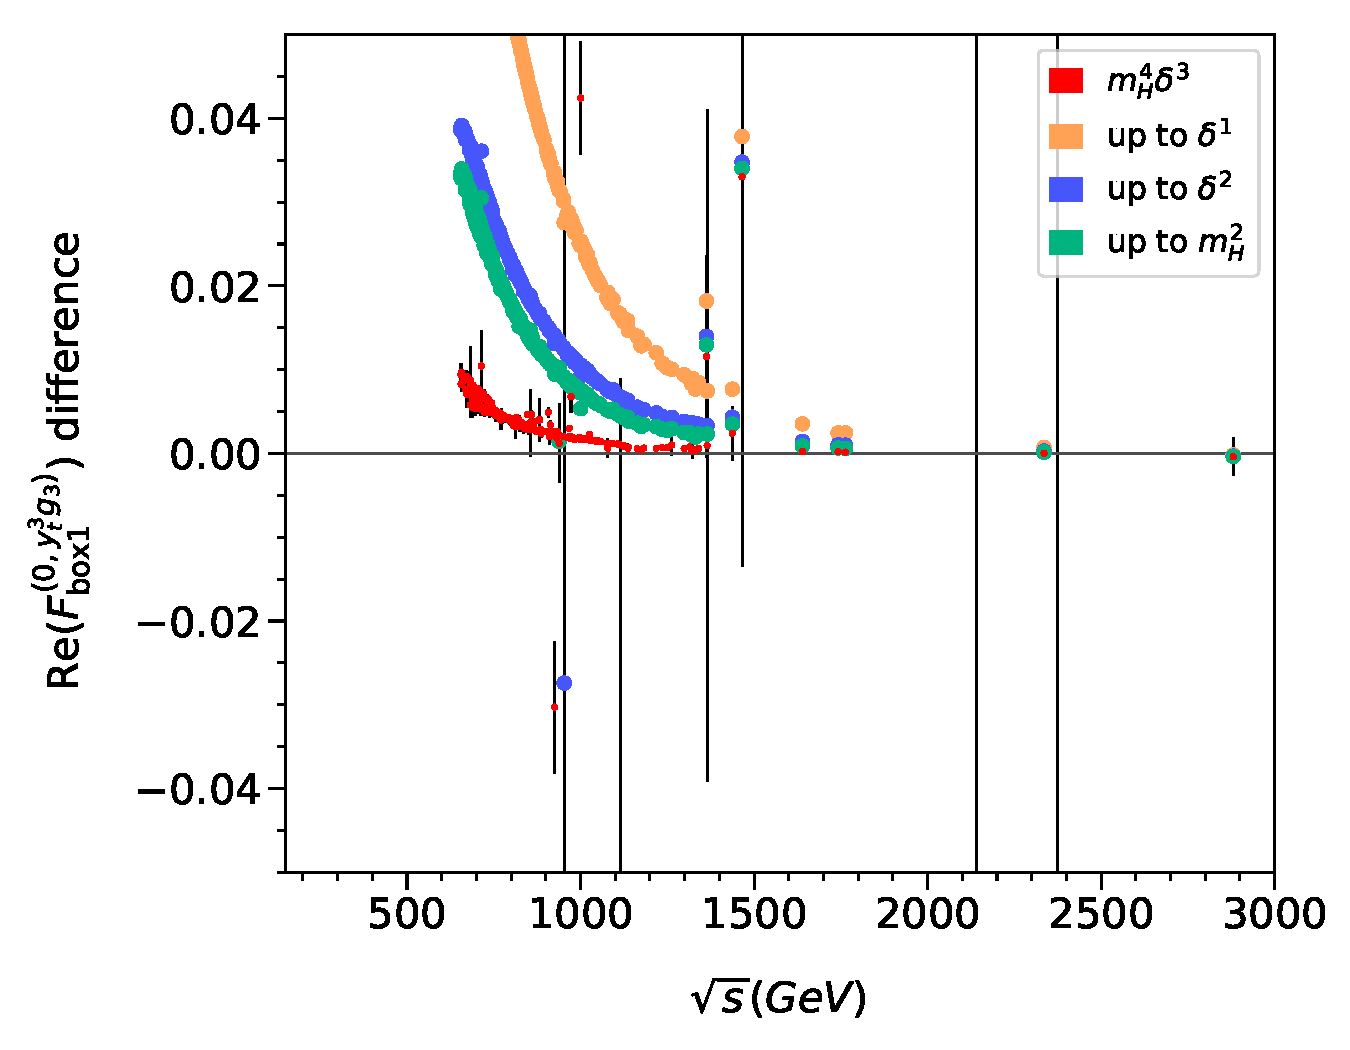
\includegraphics[width=0.48\textwidth]{NLO_EW_SM/EW_top-Higgs_self/Images/diff_to_SD_F1bare_ep0_t-plus_mhs2del3_yt3lam1_pTcut300_re_sqrts}}}
	\quad
    \subfloat[]{{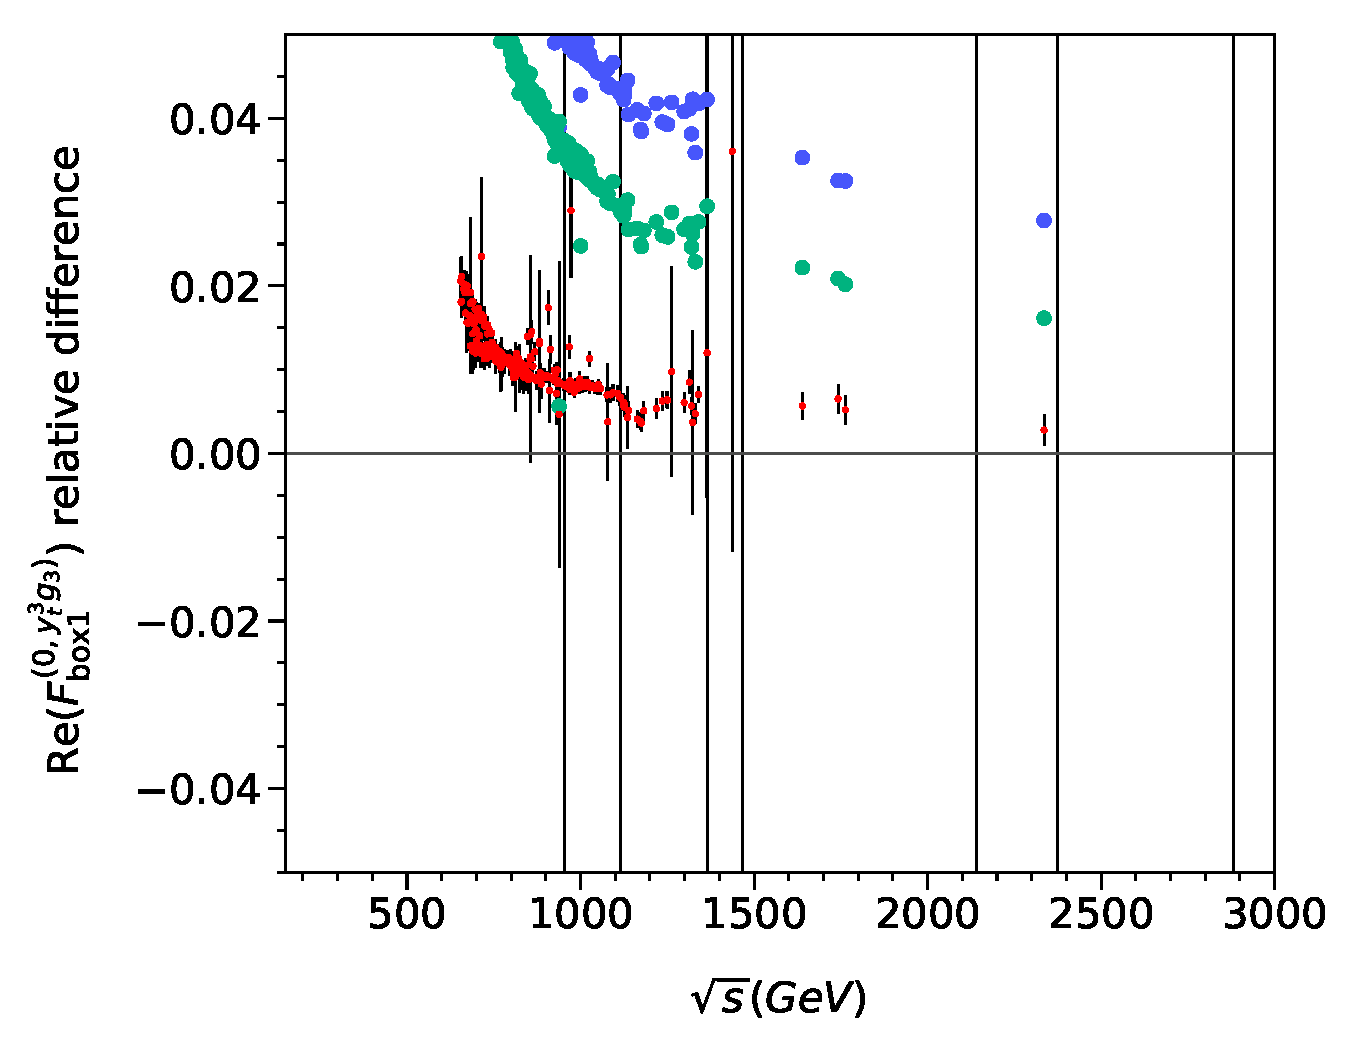
\includegraphics[width=0.48\textwidth]{NLO_EW_SM/EW_top-Higgs_self/Images/diff_to_SD_F1bare_ep0_t-plus_mhs2del3_yt3lam1_pTcut300_re_sqrts_rel}}}
	\caption{Real part of the form factor (a) from Feynman diagrams like those shown in Fig.~\ref{fig::diags}. (b) and (c) show the absolute and relative difference compared to Ref.~\cite{Heinrich:2024dnz}. Analytic results shown are from Ref.~\cite{Davies:2025wke}.}
    \label{fig::diff_to_SD_yt3lam1}
\end{figure}


\begin{figure}
\centering
    \subfloat[]{{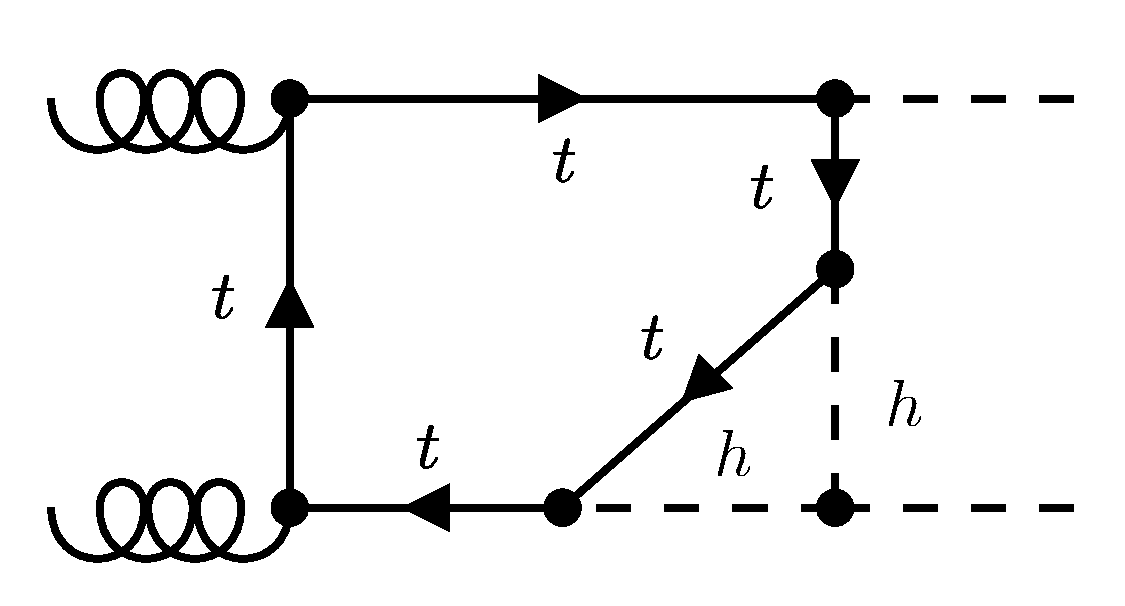
\includegraphics[width=0.3\textwidth]{NLO_EW_SM/EW_top-Higgs_self/Images/gghh_c_h.pdf}}}
	\quad
    \subfloat[]{{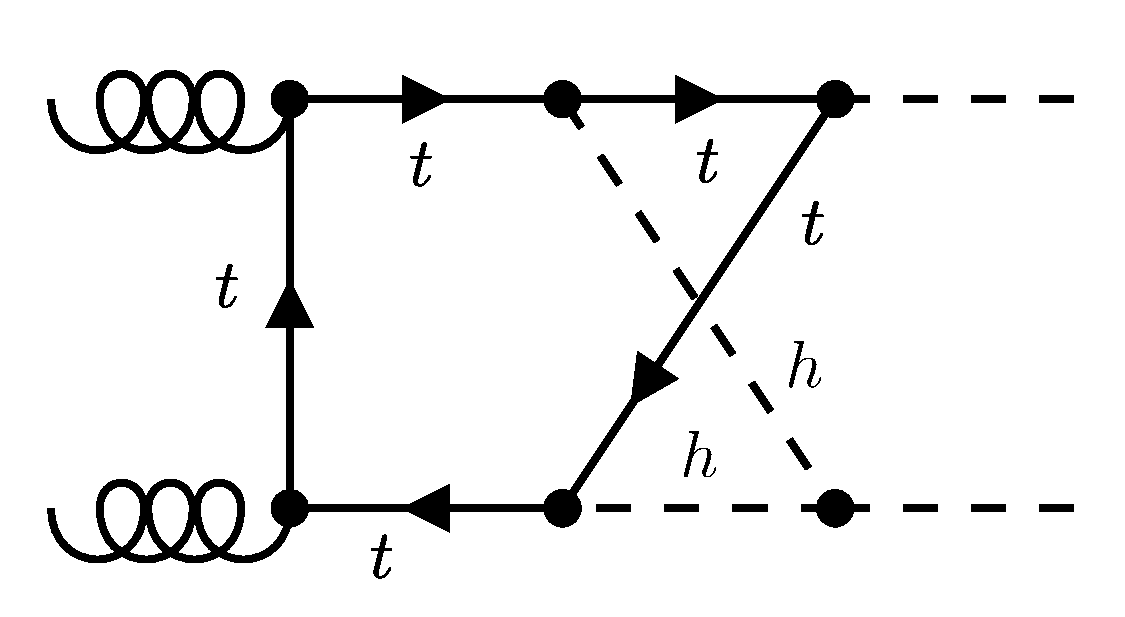
\includegraphics[width=0.3\textwidth]{NLO_EW_SM/EW_top-Higgs_self/Images/gghh_e_h.pdf}}}
	\caption{Sample Feynman diagrams. Solid, dashed and curly lines represent top quarks, Higgs bosons and gluons, respectively. Diagrams from Ref.~\cite{Davies:2025wke}.}
    \label{fig::diags}
\end{figure}


~

\noindent \textbf{Gudrun Heinrich, Stephen Jones, Matthias Kerner, Thomas Stone, Augustin Vestner~\cite{Heinrich:2024dnz}.}

\noindent In Ref.~\cite{Heinrich:2024dnz}, fully differential results for the Yukawa- and Higgs boson self-coupling-type electroweak corrections to Higgs boson pair production in gluon fusion are presented.
The results retain the full dependence on the mass of the top quark and the Higgs boson.
At the amplitude level, the results are further separated into the individual coupling structures, allowing for the bare amplitude to be computed with arbitrary top Yukawa coupling, trilinear Higgs boson self-coupling, and quartic Higgs boson self-coupling.

The precise class of corrections which are computed is defined via a Yukawa model with only an up-type quark (the top quark) and a scalar field (the Higgs boson). Example Feynman diagrams are shown in Fig.~\ref{fig:240704653_examplediags}.
This model selects a well-defined subset of diagrams which can be obtained from considering the SM in the unitary gauge and then setting $(g, g^\prime) \rightarrow (0,0)$, which removes the electroweak gauge bosons (and their associated ghost fields).
The electroweak input-parameter scheme $\left\{ M_Z=0, M_W=0, G_F\right\}$ + $\left\{m_t,m_h\right\}$ is used, where all masses are specified in the on-shell scheme.
Results are presented with the Higgs vev fixed in the $G_\mu$ scheme (with $M_Z=0$, $M_W=0$). However, the intermediate results are sufficiently general to allow another renormalization scheme to be adopted.
Tadpole contributions are treated within the Fleischer--Jegerlehner tadpole scheme (FJTS)~\cite{Fleischer:1980ub}.


\begin{figure}
\centering
    \subfloat[]{{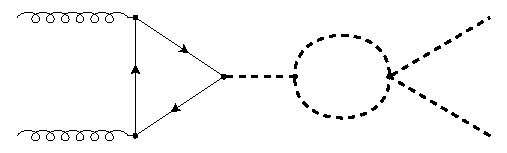
\includegraphics[width=0.3\textwidth]{NLO_EW_SM/EW_top-Higgs_self/Images/NLOtritpropHbubH}}}
	\qquad
    \subfloat[]{{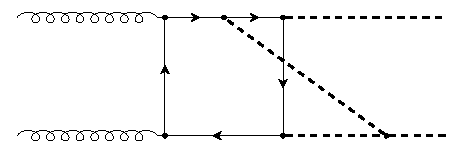
\includegraphics[width=0.3\textwidth]{NLO_EW_SM/EW_top-Higgs_self/Images/NLOboxHvertcorr}}}
	\qquad
    \subfloat[]{{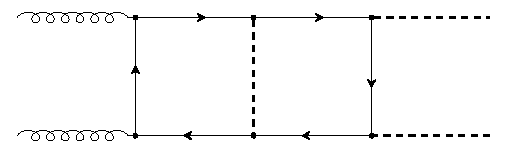
\includegraphics[width=0.3\textwidth]{NLO_EW_SM/EW_top-Higgs_self/Images/NLOboxtboxt}}}
		\caption{Example diagrams contributing to the different coupling structures into which the bare two-loop amplitude is separated. Diagrams from Ref.~\cite{Heinrich:2024dnz}.}
    \label{fig:240704653_examplediags}
\end{figure}


The calculation is performed by projecting the bare amplitude onto the two form factors described above in $D=4-2\epsilon$ dimensions.
The unreduced amplitude is obtained using two separate calculations based on either \texttt{alibrary}~\cite{alibrary}, a \texttt{Mathematica} and \texttt{Form}~\cite{Kuipers:2013pba} package for computing multi-loop amplitudes, or \texttt{Reduze 2}~\cite{vonManteuffel:2012np}, allowing for a detailed cross-check.
The form factors are then reduced fully symbolically, retaining the dependence on the Mandelstam invariants ($s$, $t$), the masses ($m_h$, $m_t$) and the space-time dimension $D$, to a basis of 494 finite master integrals using the public programs \texttt{Kira}~\cite{Klappert:2020nbg}, \texttt{Ratracer}~\cite{Magerya:2022hvj}, and \texttt{Firefly}~\cite{Klappert:2019emp,Klappert:2020aqs}.
The master integrals appearing in the reduced form factors are then evaluated numerically for each phase-space point using \texttt{pySecDec}~\cite{Borowka:2017idc,Borowka:2018goh,Heinrich:2021dbf,Heinrich:2023til}. The evaluation of the master integrals is additionally cross-checked at several physical points using \texttt{DiffExp}~\cite{Hidding:2020ytt,Moriello:2019yhu}.


\begin{figure}
\centering
    \subfloat[]{{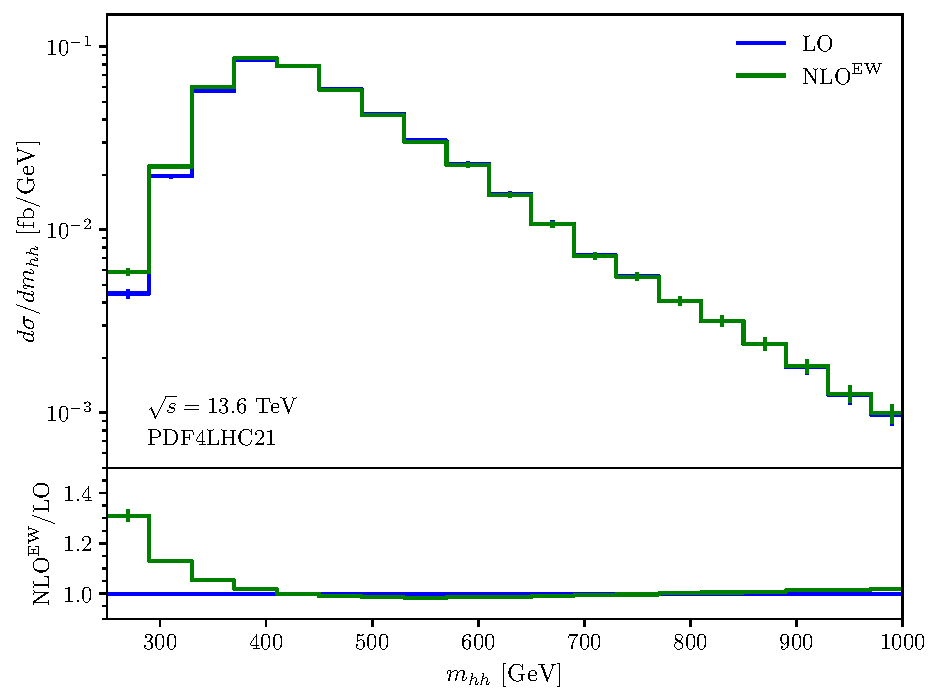
\includegraphics[width=0.48\textwidth]{NLO_EW_SM/EW_top-Higgs_self/Images/mhh_full_h.pdf}}}
	\quad
    \subfloat[]{{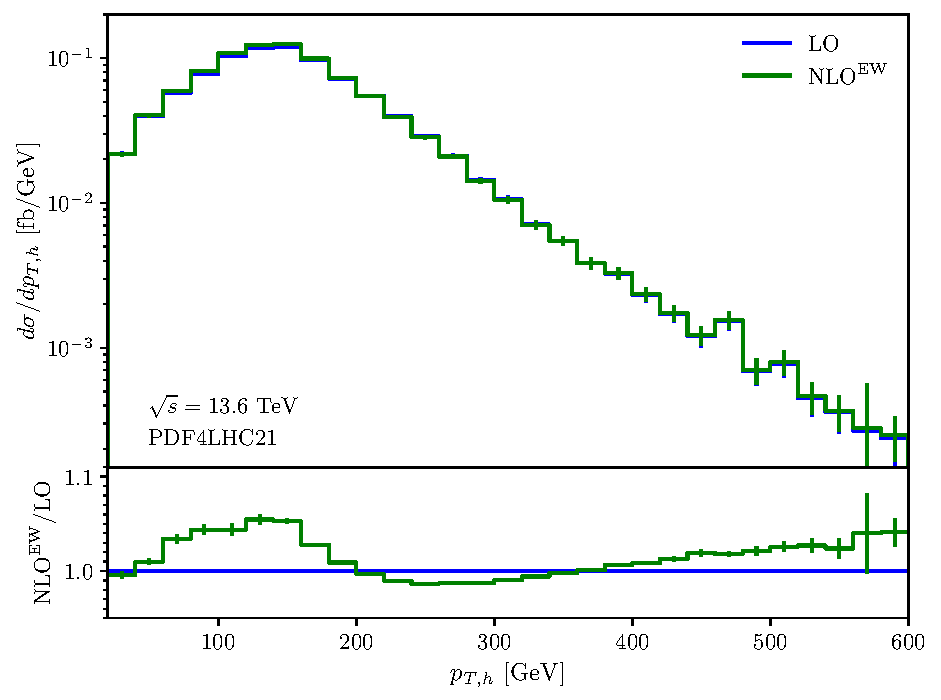
\includegraphics[width=0.48\textwidth]{NLO_EW_SM/EW_top-Higgs_self/Images/pth_full_h.pdf}}}
    \caption{Invariant mass (a) and transverse momentum (b) distributions for Higgs boson pair production at LO and $\mathrm{NLO}^\mathrm{EW}$ including only the Yukawa and Higgs boson self-coupling-type corrections. Results shown are from Ref.~\cite{Heinrich:2024dnz}.}
    \label{fig:240704653_dists}
\end{figure}


In Fig.~\ref{fig:240704653_dists}, results for the Higgs boson pair invariant mass and $p_{T,H}$~distribution are shown.
The results presented here are obtained using the \texttt{PDF4LHC21\_40}~\cite{PDF4LHCWorkingGroup:2022cjn} parton distribution functions interfaced via \texttt{LHAPDF}~\cite{Buckley:2014ana} and setting the factorization and renormalization scale to $\mu_r = \mu_f = m_{hh}/2$. The masses of the Higgs boson and top quark are set to $m_h = 125~\mathrm{GeV}$, $m_t = \sqrt{23/12}\,m_h = 173.055$ GeV, respectively, and $G_F = 1.1663787 \cdot 10^{-5}\,\textup{GeV}^{-2}$, corresponding to $v=246.22~\mathrm{GeV}$.
For the subset of the electroweak correction considered, very large shape distortions (around $30\%$ for the binning selected) are observed close to threshold for the invariant mass distribution, with much smaller corrections above $400\,\textup{GeV}$ (up to $1\,\textup{TeV}$).
The corrections in the $p_{T,H}$ distribution are less localized, with distortions of up to $5\%$ present across the spectrum.
Overall, the top Yukawa and Higgs boson self-coupling corrections amount to a $1\%$ enhancement of the total cross section.

An important observation concerns the renormalizability of models in which the top Yukawa coupling, the trilinear Higgs boson self-coupling, and the quartic Higgs boson self-coupling are varied from their SM values.
In particular, it is observed that the $1/\epsilon$ pole structure of the vev counterterm obtained by demanding the finiteness of the Yukawa or Higgs boson self-coupling vertices differs unless they are each set to their SM value.
This implies that the $\kappa$-framework used to extract the trilinear Higgs boson self-coupling modifier, $\kappa_\lambda \equiv \lambda_{hhh}/\lambda_{hhh}^{\rm SM}$, cannot directly be used when including the electroweak corrections to this process.
Furthermore, even though the quartic Higgs boson self-coupling first enters at $\mathrm{NLO}_\mathrm{EW}$, the subset of diagrams in which it appears is divergent prior to UV renormalization, implying that the $\kappa_4$ coupling also cannot naively be varied.


\subsubsection{Light-quark contributions}

\label{EW:light-quark}

%\paragraph{Authors:}
%\begin{itemize}
%    \item Marco Bonetti, Philipp Rendler, William J. Torres Bobadilla~\cite{Bonetti:2025vfd,BoHeReToBa_TBA};
%    \item Arunima Bhattacharya, Francisco Campanario, Sauro Carlotti, Jamie Chang, Javier Mazzitelli, Margarete Mühlleitner, Jonathan Ronca, Michael Spira ~\cite{Bhattacharya_TBA}.
%\end{itemize}


\begin{figure}
\centering
    \subfloat[$VVh$]{{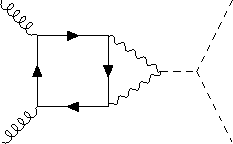
\includegraphics[height=0.10\textheight]{NLO_EW_SM/EW_light_quarks/Images/gg-HHH}}\label{fig:VVHV}}
	\qquad\qquad
    \subfloat[$VVhh$]{{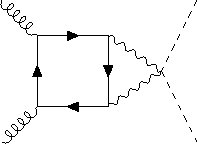
\includegraphics[height=0.10\textheight]{NLO_EW_SM/EW_light_quarks/Images/gg-HHVV}}\label{fig:HHVV}}
	\qquad\qquad
    \subfloat[$VVV$]{{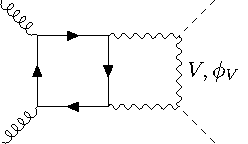
\includegraphics[height=0.10\textheight]{NLO_EW_SM/EW_light_quarks/Images/gg-VVV}}\label{fig:VVV}}
	\caption{Representative diagrams for the light-quark contributions from Ref.~\cite{Bonetti:2025vfd}.}
    \label{fig:amplgg}
\end{figure}


Double Higgs boson production in gluon fusion mediated by light quarks appears for the first time at two loops: the gluons couple to a light-quark box, to which either two $W$ or two $Z$ bosons are attached, subsequently generating the Higgs boson(s). Three blocks of contributions can be identified: one-particle reducible diagrams containing one vector-vector-Higgs vertex and one trilinear Higgs boson self-coupling vertex (dubbed $VVH$, see Fig.~\ref{fig:VVHV}); diagrams containing a vector-vector-Higgs-Higgs vertex ($VVHH$, Fig.~\ref{fig:HHVV}); and diagrams containing two vector-vector-Higgs vertices ($VVV$, Fig.~\ref{fig:VVV}).\footnote{The $VVV$ type of diagrams may also contain a Goldstone boson connecting the two Higgs bosons.} Each one of these blocks is further divided into diagrams containing either $W$ or $Z$ bosons only. Each one of the aforementioned terms is explicitly gauge-invariant and UV- and IR-finite. Four light flavours are considered in diagrams containing $W$ bosons, while five light flavours have been taken into account in diagrams containing $Z$ bosons.

~

\noindent \textbf{Marco Bonetti, Philipp Rendler, William Torres Bobadilla~\cite{Bonetti:2025vfd}.}

\noindent In Ref.~\cite{Bonetti:2025vfd} fully symbolic expressions for each of the blocks described above have been calculated. The amplitude has been decomposed as a linear combination of the standard tensors $T_1^{\mu\nu}$ and $T_2^{\mu\nu}$ of Section~\ref{intro_ampli}.\footnote{No axial terms are generated by the fermion loop thanks to charge-parity conservation.}

The two form factors are extracted, and the set of scalar two-loop Feynman integrals appearing there is reduced to master integrals. Differential equations are derived for specific linear combinations of the master integrals with respect to the Mandelstam variables and the masses, such that their solution can be written in terms of iterated integrals over logarithmic kernels. This choice of basis is further improved by applying a series of rotations to eliminate redundant integration kernels. Integration constants are fixed by matching the expressions of the master integrals to their large-$m_{W,Z}$ expansion.

The results are employed to obtain analytic expressions for the form factors, further identifying independent functions therein for which dedicated differential equations are built for optimized numerical evaluation in terms of generalized series expansions evolved from the large-mass limit to arbitrary points in the physical region of the phase space. A code implementation for the numerical evaluation of the functions is provided, based on the \texttt{Mathematica} package \texttt{DiffExp}~\cite{Hidding:2020ytt}. Grids for the light-quark amplitude, as well as for its interference with the LO amplitude, have been implemented in the POWHEG-BOX framework or are available upon request. The interference between the LO amplitude and the first form factor of the light-quark amplitude represents the main source of contributions except for the high-energy tail, where the second form factor becomes relevant, although very small overall. Large cancellations occur when considering the interference between LO triangle and box diagrams with each of the $VVh$, $VVhh$, and $VVV$ blocks, suggesting that the light-quark terms are highly sensitive to variations of the trilinear Higgs boson self-coupling.


\begin{figure}
\centering
    \subfloat[]{{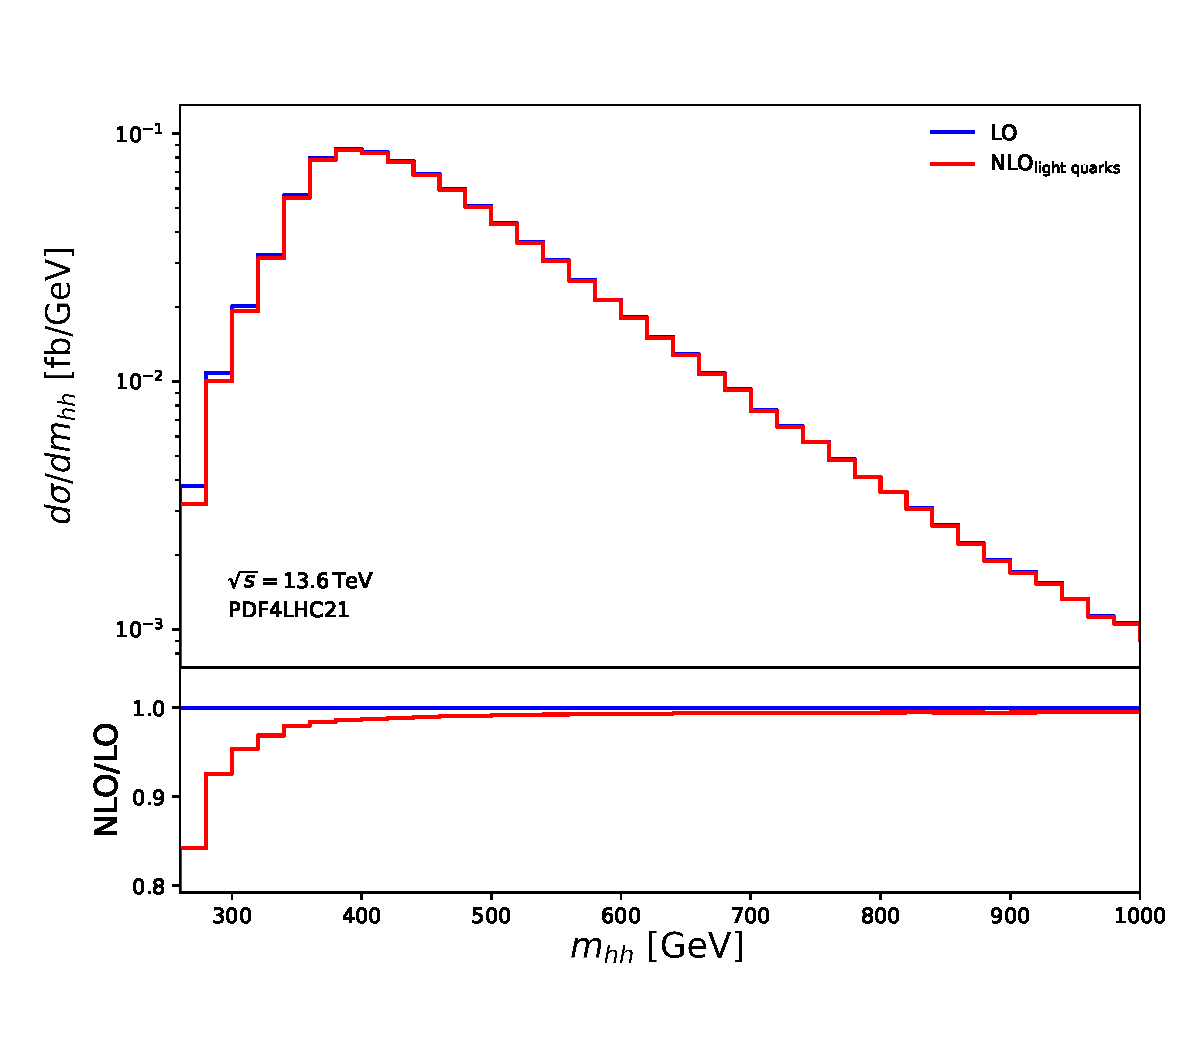
\includegraphics[width=0.48\textwidth]{NLO_EW_SM/EW_light_quarks/Images/mhh2_hfix.pdf}}\label{fig:lq_mHH}}
	\quad
    \subfloat[]{{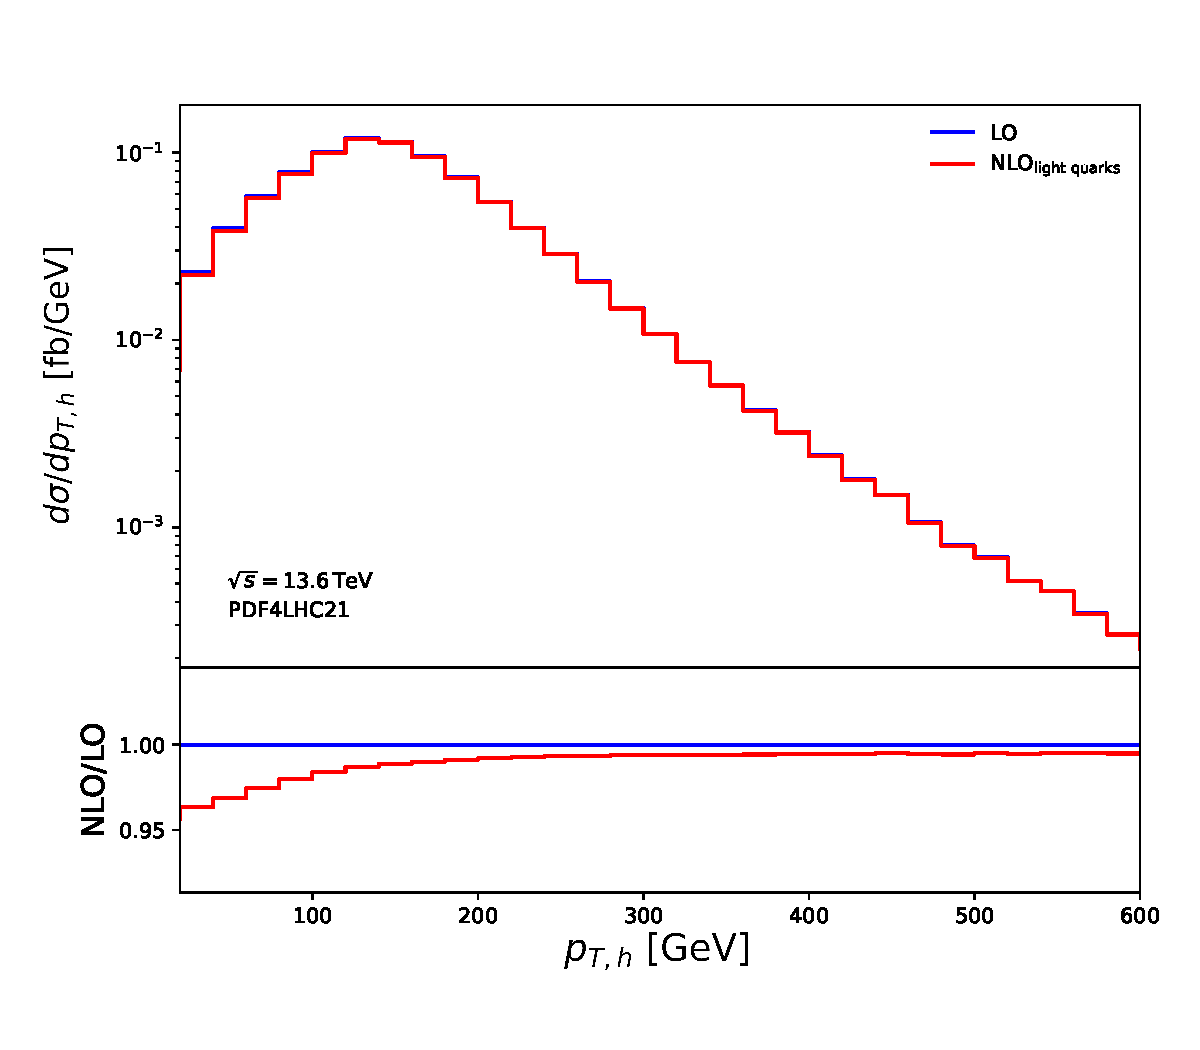
\includegraphics[width=0.48\textwidth]{NLO_EW_SM/EW_light_quarks/Images/pt_hfix.pdf}}\label{fig:lq_pTH}}
	\caption{Light-quark and Yukawa contributions to the Higgs boson pair invariant mass (a) and Higgs transverse momentum distributions (b).}
    \label{fig:lq_obs}
\end{figure}


The impact of the light-quark corrections to the Higgs boson pair invariant mass distribution and the transverse momentum distribution is depicted in Figs.~\ref{fig:lq_mHH} and~\ref{fig:lq_pTH}, respectively. The light-quark corrections suppress both the invariant mass and the transverse momentum distribution at all centre-of-mass energies, with particular relevance for the region of the phase space close to the production threshold, where they have a negative effect of more than $-15\%$ on the $m_{hh}$ distribution and around $-4\%$ on the $p_{T,h}$ distribution. In both cases, the corrections quickly approach zero as the centre-of-mass energy grows.

~

\noindent \textbf{Arunima Bhattacharya, Francisco Campanario, Sauro Carlotti, Jamie Chang, Javier Mazzitelli, Milada Margarete Mühlleitner, Jonathan Ronca, Michael Spira ~\cite{Bhattacharya_TBA}.}

\noindent Ref.~\cite{Bhattacharya_TBA} provides an independent evaluation of the light-quark contributions to $gg \to hh$. The bottleneck of this calculation is the evaluation of the genuine two-loop box diagrams $VVV$ (see Fig.~\ref{fig:VVV}). The numerical stability of these diagrams is quite demanding, since strong cancellations emerge between all diagrams, which require the form factors of the individual diagrams to be numerically determined with very significant precision. The numerical method applied to these diagrams is the same as in Section~\ref{EW:Top-Higgs_sector}, i.e.\ projection on the two form factors of Eq.~\eqref{eq:FFdeco} in $D=4-2\epsilon$ dimensions, no tensor reduction, Feynman parametrization and analytical continuation of all propagator masses including the $W$ and $Z$ boson masses, $M_{W/Z}^2 \to M_{W/Z}^2 (1-i\bar\epsilon)$. To isolate the singularities, multiple end-point subtractions need to be performed. In order to reach the narrow-width limit $\bar\epsilon\to 0$, a Richardson extrapolation was performed with a minimal regulator down to $\bar\epsilon = 0.025$ depending on $m_{hh}$.

The two-loop triangle diagrams $VVh$ (see Fig.~\ref{fig:VVHV}) can be adopted from the single-Higgs calculation \cite{Aglietti:2004nj,Aglietti:2006yd} and translated to the two-loop box diagrams with a 4-point vertex $VVhh$ (see Fig.~\ref{fig:HHVV}).


\begin{figure}[!hbtp]
    \centering
   % \vspace*{-3.2cm}
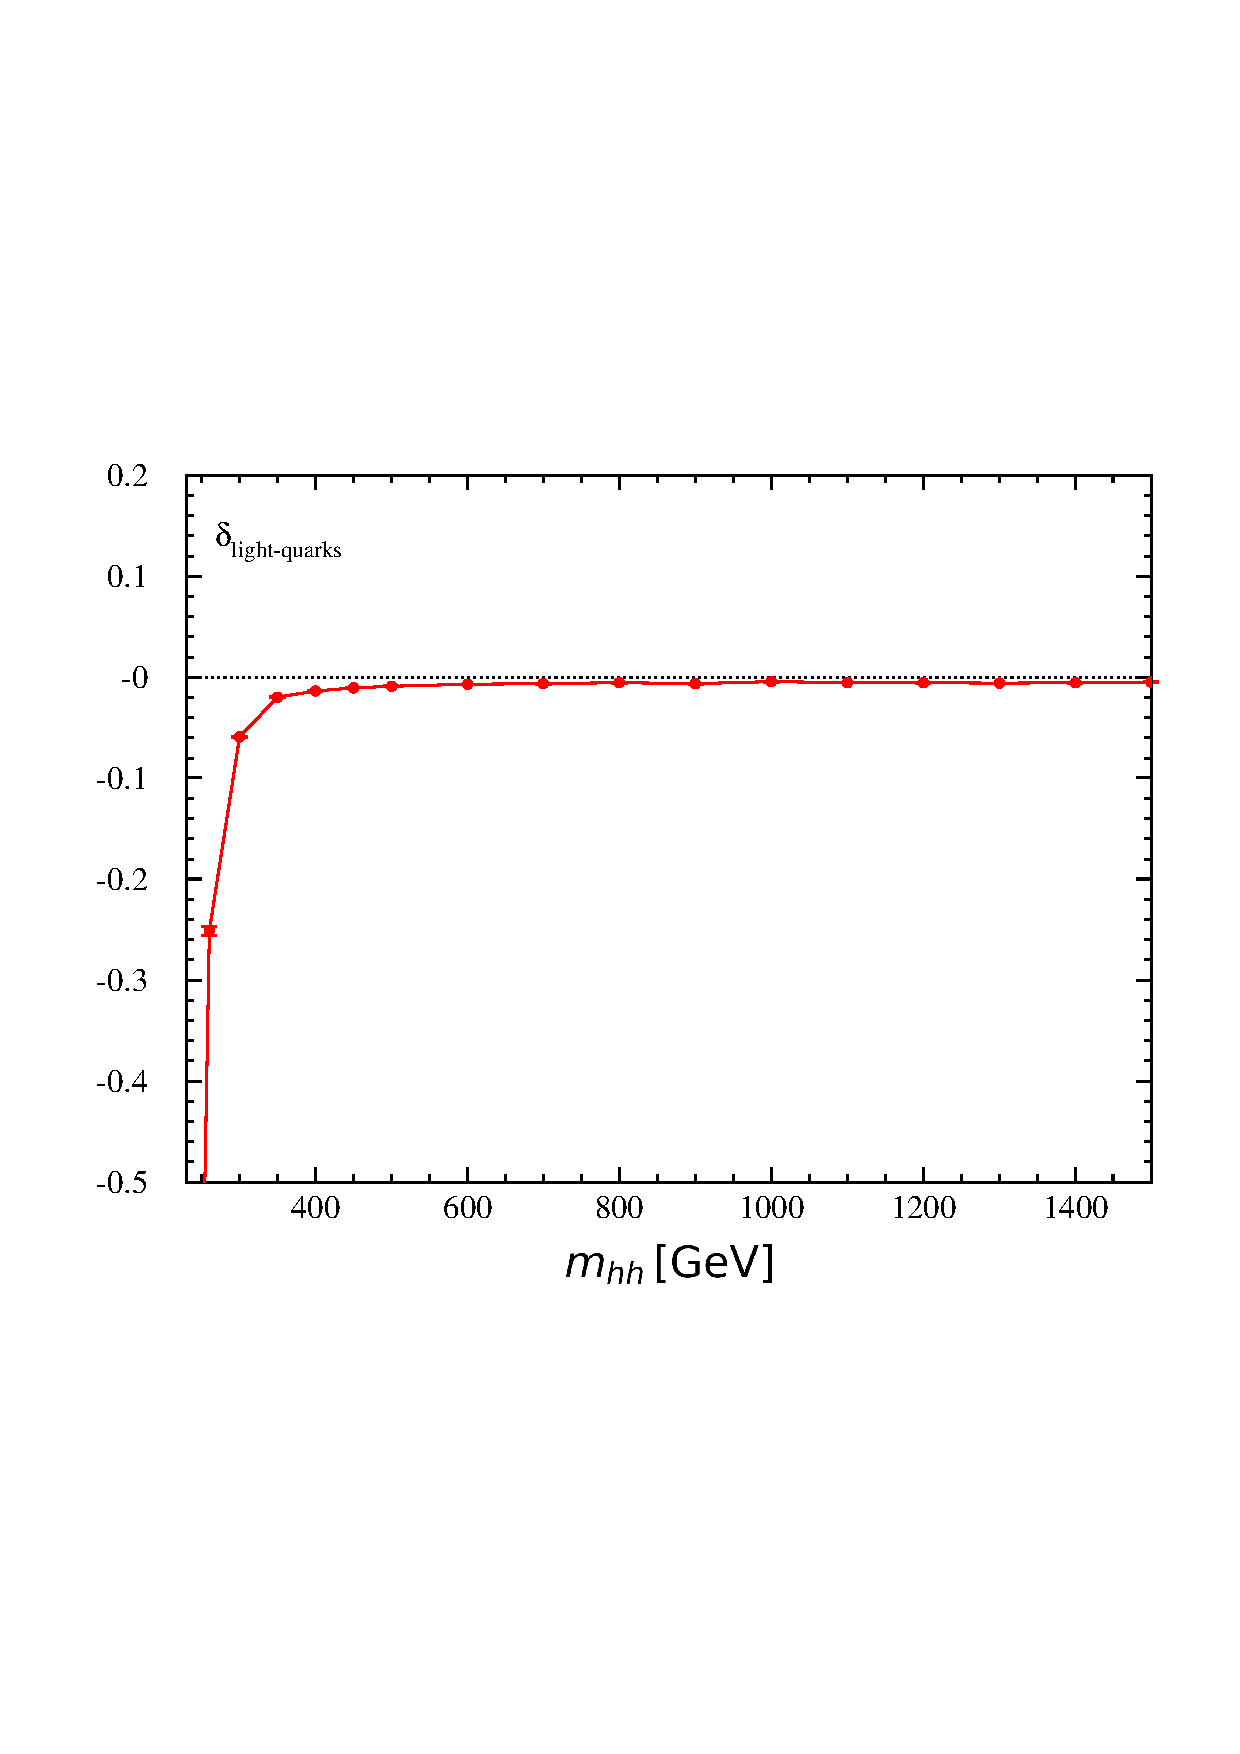
\includegraphics[width=0.48\textwidth]{NLO_EW_SM/EW_light_quarks/Images/delta_lq_hfix.pdf}
 %   \vspace*{-3.2cm}
\caption{\label{fg:delta_lq}The full relative light-quark loop-induced electroweak corrections to the $gg \to hh$ process. The points on the curve together with their numerical error bars indicate the $m_{hh}$ values for which the corrections have been computed. Results shown are from Ref.~\cite{Bhattacharya_TBA}.}
\end{figure}


The total sum of all light-quark loop diagrams is finite, and no renormalization is required. The result is a small correction at the sub-percent level for large values of $m_{hh}$, see Fig.~\ref{fg:delta_lq}, while the corrections are larger close to the production threshold due to the cancellation of the leading top quark mass terms of the LO matrix element, to which the results are normalized. In total, the light-quark loops do not play a dominant role in Higgs boson pair production via gluon fusion in contrast to single-Higgs production \cite{Actis:2008ts,Actis:2008ug}.

~

\paragraph{Comparison.}

The two independent evaluations of the light-quark contributions mentioned above have been found to agree within the numerical uncertainties.




\subsection{Quark-antiquark-initiated contributions}

\label{EW:qqbar}

A Higgs boson pair can also be produced in the quark-antiquark channel. The Higgs bosons can be generated either through direct Yukawa couplings to massive bottom quarks or through intermediate EW vector bosons. Direct Yukawa production already occurs at tree level but is suppressed by the small Yukawa couplings, while EW-boson-mediated production is loop-induced.



\noindent \textbf{Marco Bonetti, Gudrun Heinrich, Philipp Rendler, William  Torres~Bobadilla~\cite{Bonetti:2026cih}.}


\begin{figure}
\centering
    \subfloat[LO.]{{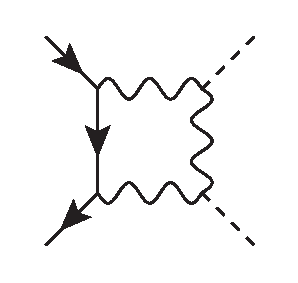
\includegraphics[height=0.10\textheight]{NLO_EW_SM/EW_qqbar_initiated/Images/VVVlo}}\label{fig:qqbarLO}}
	\qquad\qquad
    \subfloat[NLO virtual.]{{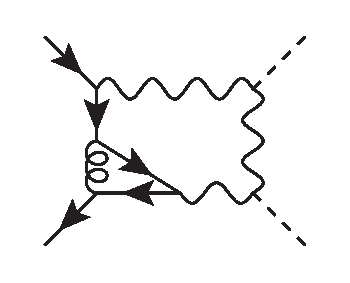
\includegraphics[height=0.10\textheight]{NLO_EW_SM/EW_qqbar_initiated/Images/VVVv}}\label{fig:qqbarV}}
	\qquad\qquad
    \subfloat[NLO real.]{{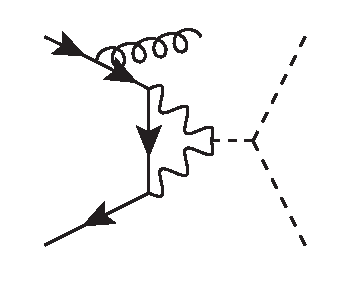
\includegraphics[height=0.10\textheight]{NLO_EW_SM/EW_qqbar_initiated/Images/HHHr}}\label{fig:qqbarR}}
	\qquad\quad

	\caption{Representative diagrams for light-quark-antiquark-initiated contributions from Ref.~\cite{Bonetti:2026cih}.}
    \label{fig:amplqqbar}
\end{figure}

\noindent The process $q\overline{q} \to hh$, mediated by weak bosons in the loop, has been calculated in Ref.~\cite{Bonetti:2026cih}, including NLO QCD corrections and considering only light quarks. Fig.~\ref{fig:amplqqbar} shows illustrative diagrams at LO and at NLO QCD. Only the first two generations of quarks are considered as initial states.

The $q\overline{q}hh$ two-loop diagrams and the $q\overline{q}hhg$ real emission diagrams contributing at NLO can be decomposed into subsets according to the number of $VVH$ or $VVhh$ vertices and vector boson propagators they contain, analogous to the light-quark contributions to $gg \to hh$ described in Section~\ref{EW:light-quark} and calculated in Ref.~\cite{Bonetti:2025vfd}.

For the two-loop virtual diagrams, only the $VVV$ subset (exemplified in Fig.~\ref{fig:amplqqbar}b) is non-zero, due to angular momentum conservation. Consequently, real emissions belonging to the $VVh$ and $VVhh$ blocks do not develop IR poles when integrating over the phase space of the unresolved extra gluon.

The one-loop amplitudes have been evaluated via the computer code \texttt{GoSam-3.0}~\cite{Braun:2025afl}, while the two-loop virtual contributions have been calculated analytically, retaining full dependence on the Mandelstam invariants and masses. The two-loop Feynman integrals have been reduced to master integrals, which have been expressed in terms of Chen iterated integrals over logarithmic kernels. Differential equations tailored to the independent transcendental functions at the level of the form factors have been constructed to produce precise numerical evaluations through the \texttt{Mathematica} package \texttt{DiffExp}~\cite{Hidding:2020ytt}.

The full set of NLO amplitudes has been implemented in the form of numerical grids in the {\tt POWHEG-BOX-V2} framework. NLO QCD corrections increase the total cross section with respect to LO $q\overline{q} \to hh$ by about $+60\%$.

On the one hand, the contribution to the total cross section coming from the quark-antiquark channel is negligible when compared to the gluon channel, amounting to about $+0.35\%$. On the other hand, the NLO QCD corrections to $q\overline{q} \to hh$ have a large shape-distorting effect at low energies in the $m_{hh}$ differential distribution, increasing the leftmost bin by about $10\%$ (cf.\ Fig.~\ref{fig:invariantMass}).\footnote{Bins with a $20\,\textup{GeV}$ width are considered.} As the low $m_{hh}$ region is also very sensitive to deviations of the trilinear Higgs boson self-coupling from the SM value, these contributions should not be neglected in high-precision predictions for Higgs boson pair production.


\begin{figure}
\centering
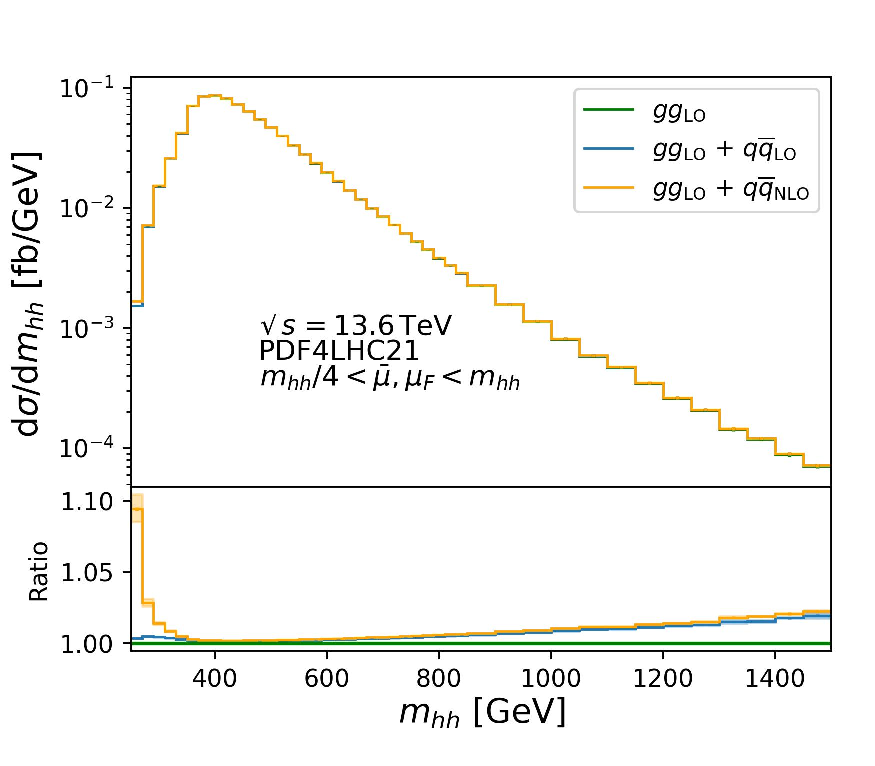
\includegraphics[width=0.49\textwidth]{NLO_EW_SM/EW_qqbar_initiated/Images/1a_HH-m_hfix.pdf}
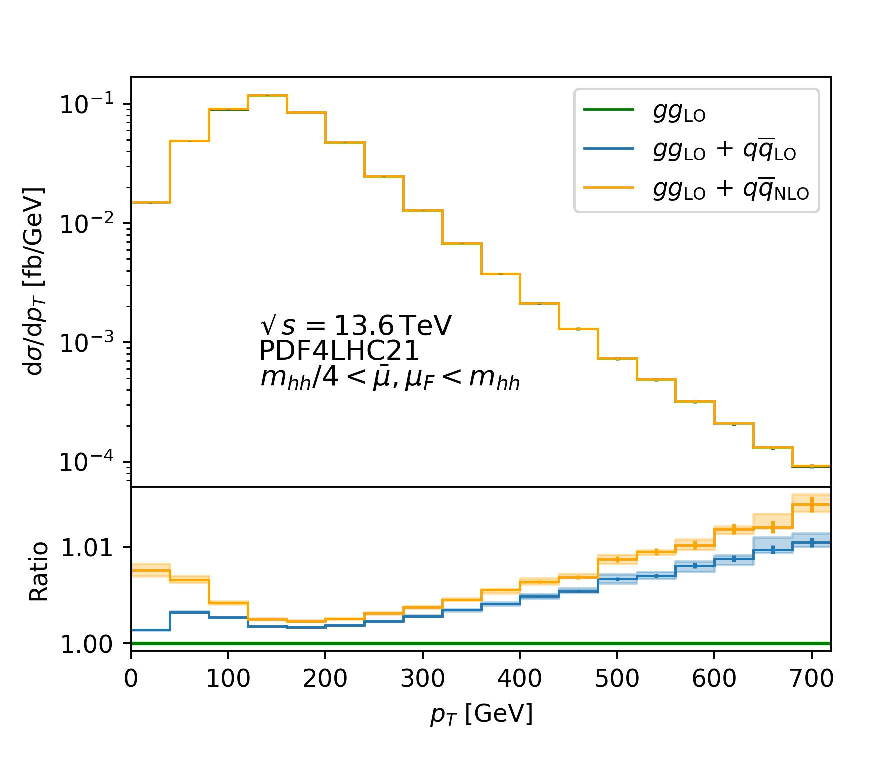
\includegraphics[width=0.49\textwidth]{NLO_EW_SM/EW_qqbar_initiated/Images/2a_H-pt_hfix.pdf}
\caption{Invariant mass distribution of the Higgs boson pair (left) and transverse momentum distribution (right) of a single Higgs boson at a proton-proton centre-of-mass energy of $\sqrt{s} = 13.6\,\textup{TeV}$. The error bands represent the scale uncertainties of the quark-antiquark channel and the error bars indicate the statistical uncertainties from the Monte Carlo integration. Figures from Ref.~\cite{Bonetti:2026cih}.
}
\label{fig:invariantMass}
\end{figure}


